\documentclass[10pt,a4paper]{article}
\usepackage[utf8]{inputenc}
\usepackage{polski}
\usepackage{amsmath}
\usepackage{amsfonts}
\usepackage{amssymb}
\usepackage{graphicx}
\usepackage{color} 
\linespread{1.3}
\addtolength{\textwidth}{3cm}
\addtolength{\hoffset}{-1.5cm}
\addtolength{\textheight}{3cm}
\addtolength{\voffset}{-1.5cm}

\begin{document}

\begin{titlepage}
	\begin{center}
    	\textbf{\Large Akademia Górniczo-Hutnicza w Krakowie} \\
    	\vspace{0.1cm}
    	{\Large Wydział Elektrotechniki, Automatyki, Informatyki i Inżynierii
    	Biomedycznej} \\
    	\vspace{1cm}
        
\includegraphics[scale = 0.4]{images/agh-logo.png} \\
        \vspace{1cm}
        \textbf{\Large PROJEKT Z PROJEKTOWANIA UKŁADÓW AUTOMATYKI PRZEMYSŁOWEJ} \\
        \vspace{1cm}
        \textbf{\Large Analiza regulatorów strojonych metodą Haalman'a} \\
        \vspace{2cm}
        {\Large Autor: Paweł Ciupek} \\
        \vfill{\Large Kraków 2016}
	\end{center}
\end{titlepage}


\section{Badane obiekty}

Badania nad proponowaną metodą strojenia regulatorów PID zostaną wykonane na obiektach o następujących transmitancjach:

\begin{equation}
P_1 = \frac{e^{-s}}{1 + sT}
\end{equation}
gdzie:\\
T = 0.02, 0.05, 0.1, 0.2, 0.3, 0.5, 0.7, 1, 1.3, 1.5, 2, 4, 6, 8, 10, 20, 50, 100, 200, 500, 1000

\begin{equation}
P_2 = \frac{e^{-s}}{1 + sT}^2
\end{equation}
gdzie:\\
T = 0.01, 0.02, 0.05, 0.1, 0.2, 0.3, 0.5, 0.7, 1, 1.3, 1.5, 2, 4, 6, 8, 10, 20, 50, 100, 200, 500

\begin{equation}
P_3 = \frac{1}{(s + 1)(1 + sT)^2}
\end{equation}
gdzie:\\
T = 0.005, 0.01, 0.02, 0.05, 0.1, 0.2, 0.5, 2, 5, 10
\begin{equation}
P_4 = \frac{1}{{(s + 1)}^n}
\end{equation}
gdzie:\\
n = 3, 4, 5, 6, 7, 8

\begin{equation}
P_5 = \frac{1}{(1 + \alpha s)(1 + \alpha^2 s)(1 + \alpha^3 s)}
\end{equation}
gdzie:\\
$\alpha$ = 0.1, 0.2, 0.3, 0.4, 0.5, 0.6, 0.7, 0.8, 0.9

\begin{equation}
P_6 = \frac{e^{-sL_1}}{s(1 + sT_1)}
\end{equation}
gdzie:\\
$L_1$ = 0.01, 0.02, 0.05, 0.1, 0.2, 0.3, 0.5, 0.7, 1\\ 
$T_1$ + $L_1$ = 1	    

\begin{equation}
P_7 = \frac{Te^{-sL_1}}{(1 + sT)(1 + sT_1)}
\end{equation}
gdzie:\\
T = 1, 2, 5, 10\\
$L_1$ = 0.01, 0.02, 0.05, 0.1, 0.2, 0.3, 0.5, 0.7, 1\\
$T_1$ + $L_1$ = 1

\begin{equation}
P_8 = \frac{1 - \alpha s}{{(s + 1)}^3}
\end{equation}
gdzie:\\
$\alpha$ = 0.1, 0.2, 0.3, 0.4 0.5, 0.6, 0.7, 0.8, 0.9, 1,  1.1

\begin{equation}
P_9 = \frac{1}{(s + 1)({(sT)}^2 + 1.4sT + 1)}
\end{equation}
gdzie:\\
T = 0.1, 0.2, 0.3, 0.4 0.5, 0.6, 0.7, 0.8, 0.9, 1
\bigskip 
\bigskip



\section{Metoda Haalman'a}

Przy wyborze nastaw regulatora PID dla obiektów, które posiadają opóźnienie L, Haalman zaproponował aby transmitancja zastępcza obiektu oraz regulatora wynosiła 

\begin{equation}
G_l = P(s)C(s) = \frac{2e^{-sL}}{3Ls}
\end{equation}\\
Stała 2/3 została dobrana poprzez minimalizacje błędu średnio kwadratowego odpowiedzi skokowej układu. Aby  dobrać nastawy regulatorów  testowane obiekty zostaną przybliżone obiektem inercyjnym I oraz II rzędu z opóźnieniem. Dla obiektu I rzędu w postaci 

\begin{equation}
P(s) = \frac{K_p e^{-sL}}{1 + sT}
\end{equation}\\
transmitancja regulatora wynosi
\begin{equation}\\
C(s) = \frac{2T}{3K_p L}(1 + \frac{1}{sT})
\end{equation}\\
Co daje regulator PI o nastawach K = 2T/3KpL oraz Ti = T. Dla obiektu II rzędu w postaci

\begin{equation}
P(s) = \frac{K_p e^{-sL}}{(1 + sT_1)(1+ sT_2)}
\end{equation}\\
Transmitancja regulatora wynosi
\begin{equation}
C(s) = \frac{2(T_1 + T_2}{3K_p L}(1 + \frac{1}{(T_1 + T_2)s} + \frac{T_1 T_2 s}{T_1 + T_2})
\end{equation}\\
Co daje regulator PID o nastawach $K = 2(T_1 + T_2)/3K_p L$, $T_i = T_1 + T_2$ oraz $T_d = T_1 T_2 / (T_1  + T_2)$

\newpage 
\section{Testy dla aproksymacji I rzędu}

Poniższe wykresy pokazują aproksymacje wszystkich obiektów obiektem inercyjnym I rzędu (na wykresach odpowiedź skokowa rzeczywistego obiektu oraz jego aproksymacji + błąd aproksymacji) oraz odpowiedzi zamkniętych układów regulacji dla wymuszenia równego 2(t) dla wszystkich stałych.\\
Parametry poszczególnych obiektów inercyjnych I rzędu zostały wyznaczone przy wykorzystaniu funkcji fmincon(), której zadaniem jest minimalizacja podanego wskaźnika jakości, którym w tym przypadku była całka z kwadratu różnicy odpowiedzi skokowej rzeczywistego obiektu oraz obiektu aproksymującego.

\newpage
\subsection{Obiekt $P_1$}
T = 0.02
\begin{center}
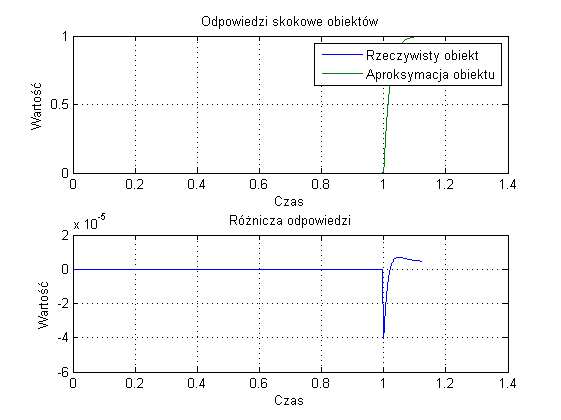
\includegraphics[scale=1]{images/jeden/skrypt_01.png}\\
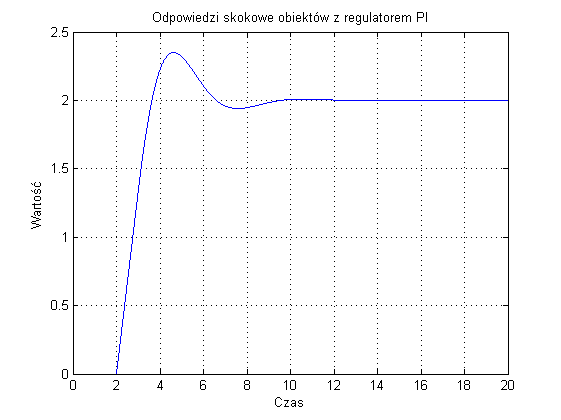
\includegraphics[scale=1]{images/jeden/skrypt_02.png}\\
\end{center}
\newpage
T = 0.05
\begin{center}
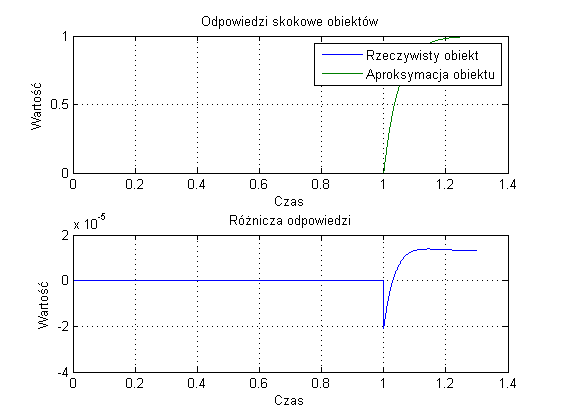
\includegraphics[scale=1]{images/jeden/skrypt_03.png}\\
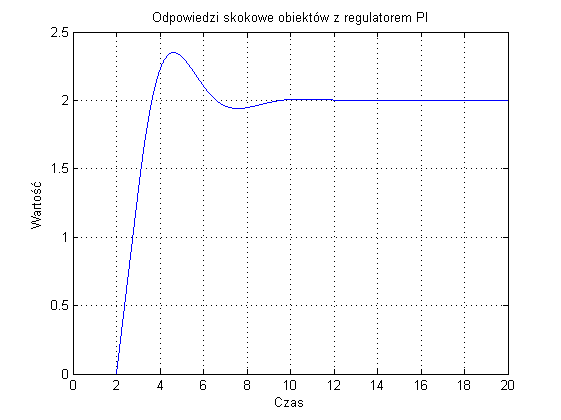
\includegraphics[scale=1]{images/jeden/skrypt_04.png}\\
\end{center}
\newpage
T = 0.1
\begin{center}
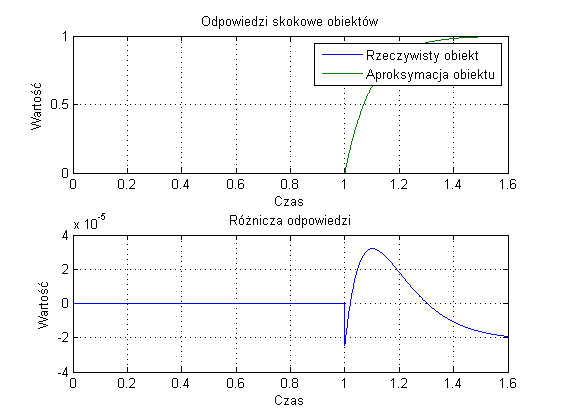
\includegraphics[scale=1]{images/jeden/skrypt_05.png}\\
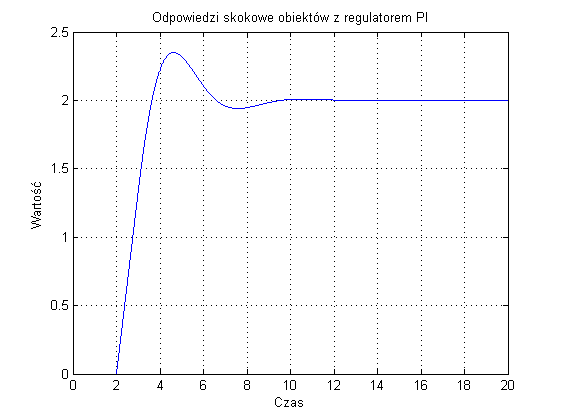
\includegraphics[scale=1]{images/jeden/skrypt_06.png}\\
\end{center}
\newpage
T = 0.2
\begin{center}
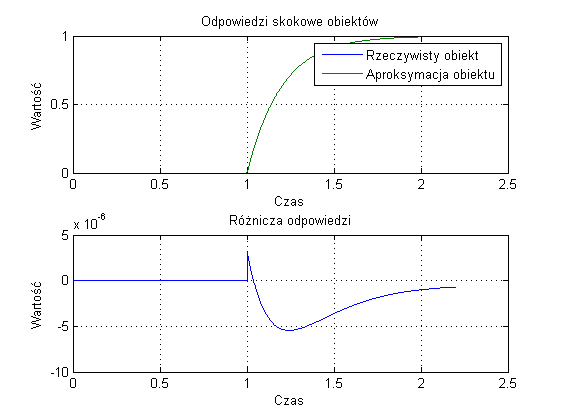
\includegraphics[scale=1]{images/jeden/skrypt_07.png}\\
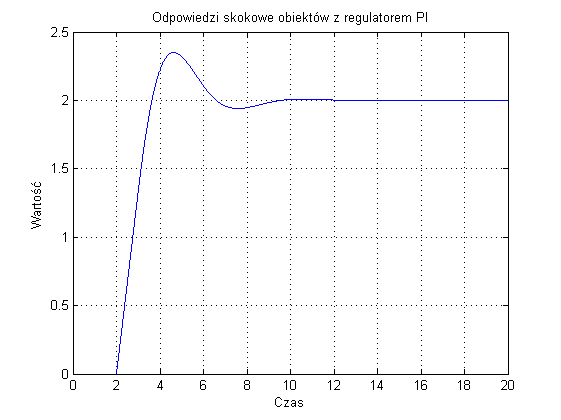
\includegraphics[scale=1]{images/jeden/skrypt_08.png}\\
\end{center}
\newpage
T = 0.3
\begin{center}
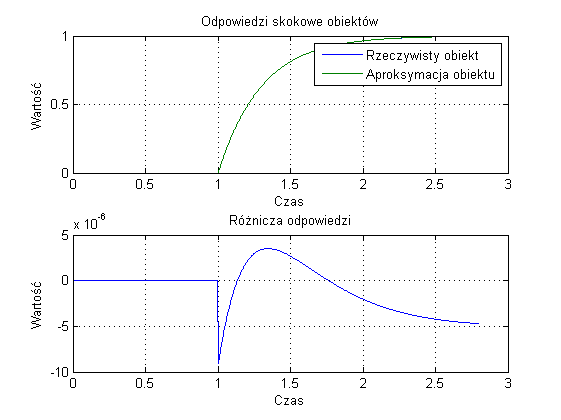
\includegraphics[scale=1]{images/jeden/skrypt_09.png}\\
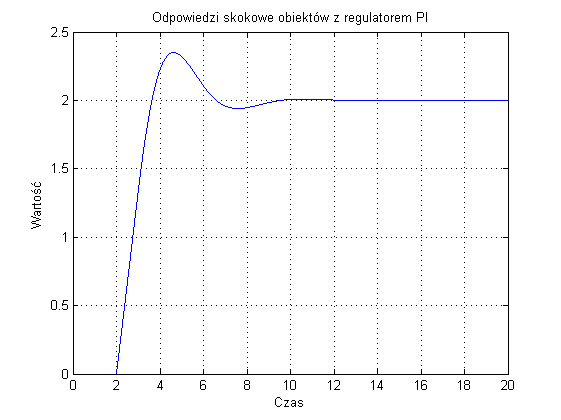
\includegraphics[scale=1]{images/jeden/skrypt_10.png}\\
\end{center}
\newpage
T = 0.5
\begin{center}
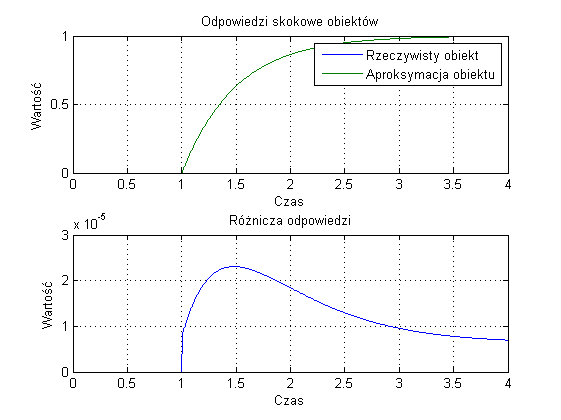
\includegraphics[scale=1]{images/jeden/skrypt_11.png}\\
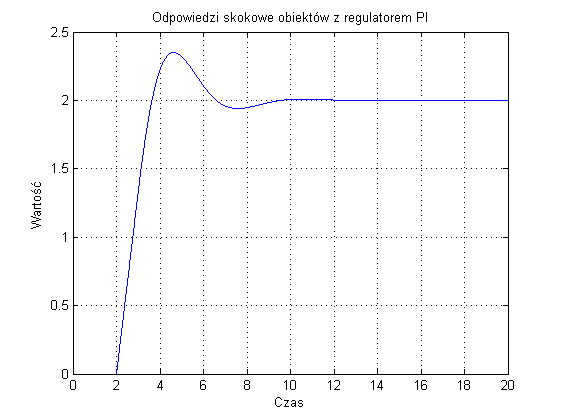
\includegraphics[scale=1]{images/jeden/skrypt_12.png}\\
\end{center}
\newpage
T = 0.7
\begin{center}
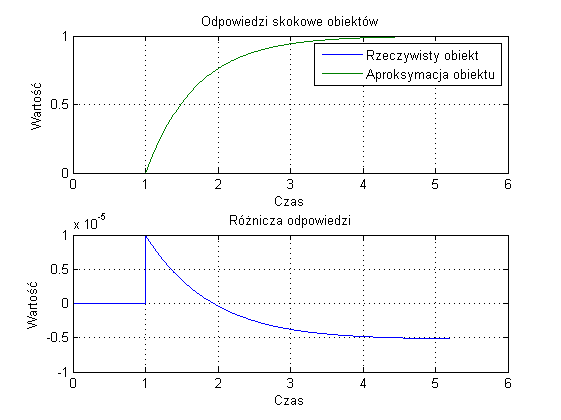
\includegraphics[scale=1]{images/jeden/skrypt_13.png}\\
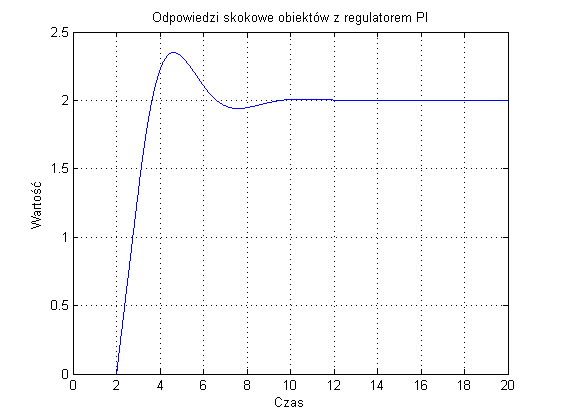
\includegraphics[scale=1]{images/jeden/skrypt_14.png}\\
\end{center}
\newpage
T = 1
\begin{center}
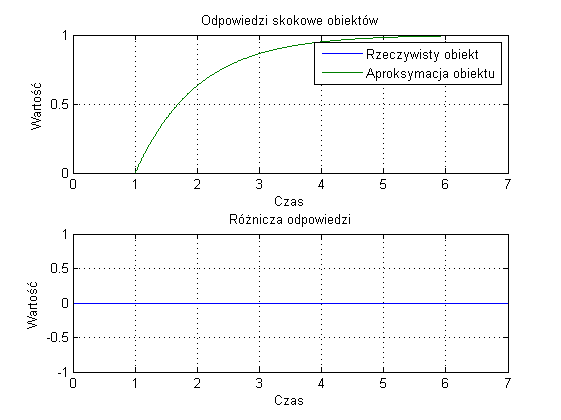
\includegraphics[scale=1]{images/jeden/skrypt_15.png}\\
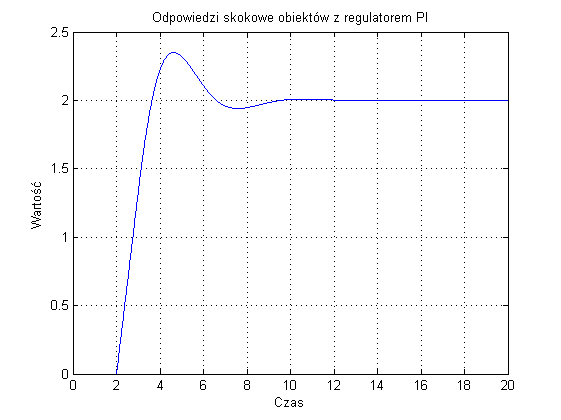
\includegraphics[scale=1]{images/jeden/skrypt_16.png}\\
\end{center}
\newpage
T = 1.3
\begin{center}
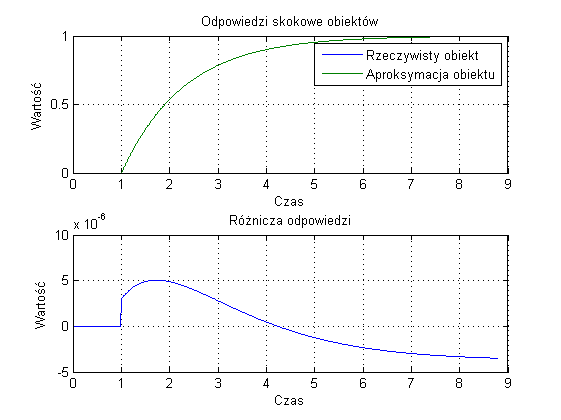
\includegraphics[scale=1]{images/jeden/skrypt_17.png}\\
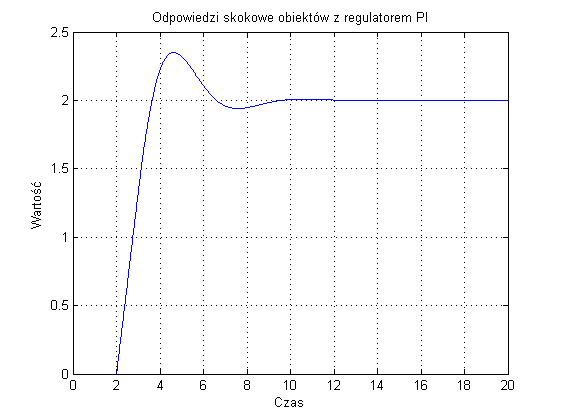
\includegraphics[scale=1]{images/jeden/skrypt_18.png}\\
\end{center}
\newpage
T = 1.5
\begin{center}
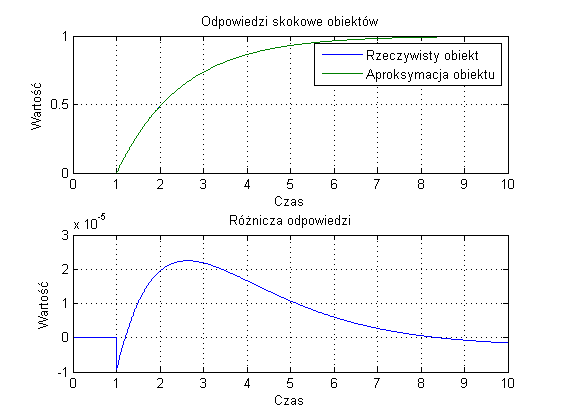
\includegraphics[scale=1]{images/jeden/skrypt_19.png}\\
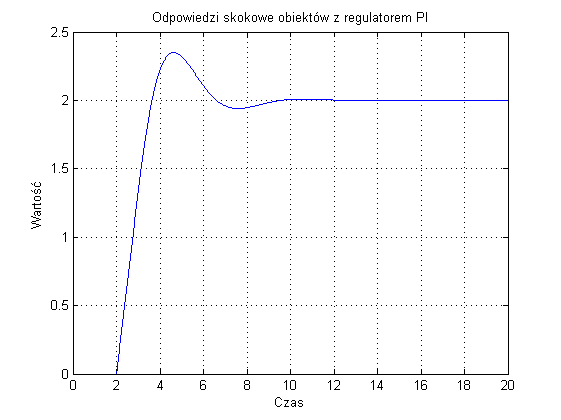
\includegraphics[scale=1]{images/jeden/skrypt_20.png}\\
\end{center}
\newpage
T = 2
\begin{center}
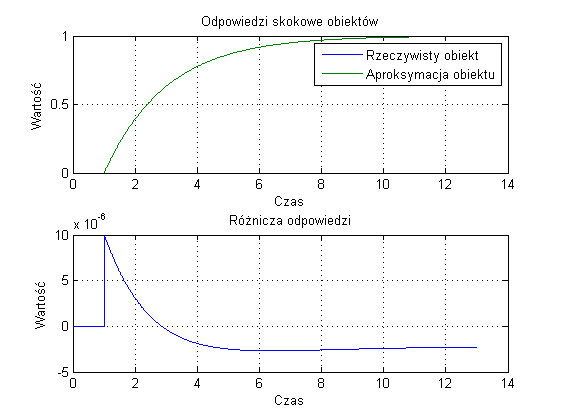
\includegraphics[scale=1]{images/jeden/skrypt_21.png}\\
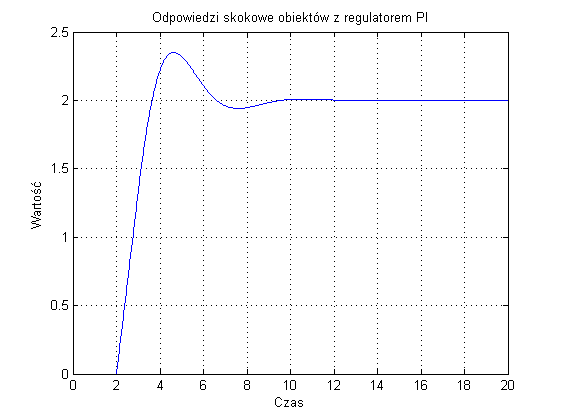
\includegraphics[scale=1]{images/jeden/skrypt_22.png}\\
\end{center}
\newpage
T = 4
\begin{center}
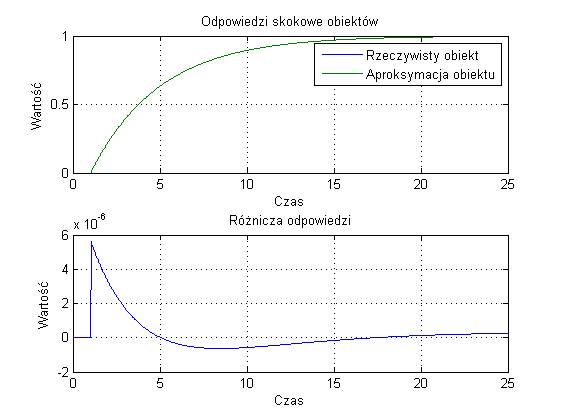
\includegraphics[scale=1]{images/jeden/skrypt_23.png}\\
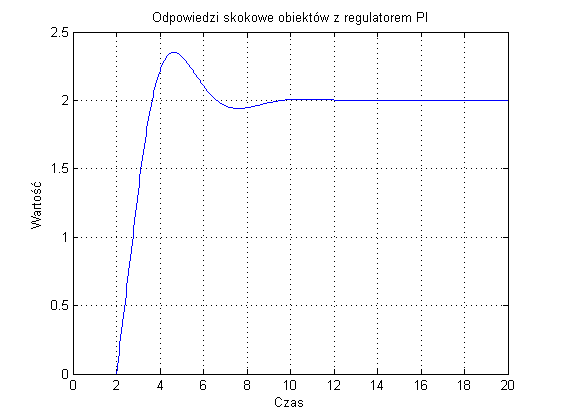
\includegraphics[scale=1]{images/jeden/skrypt_24.png}\\
\end{center}
\newpage
T = 6
\begin{center}
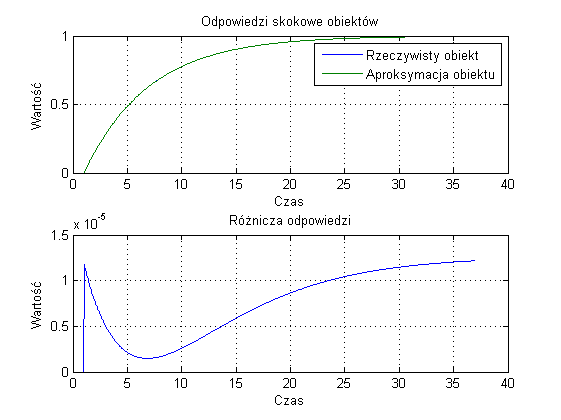
\includegraphics[scale=1]{images/jeden/skrypt_25.png}\\
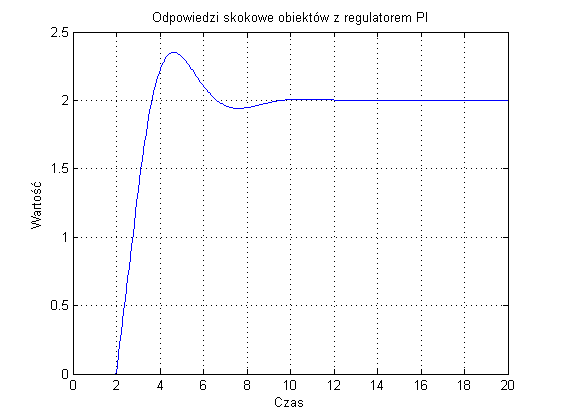
\includegraphics[scale=1]{images/jeden/skrypt_26.png}\\
\end{center}
\newpage
T = 8
\begin{center}
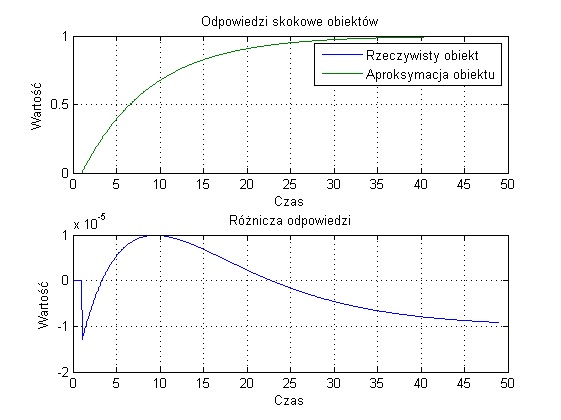
\includegraphics[scale=1]{images/jeden/skrypt_27.png}\\
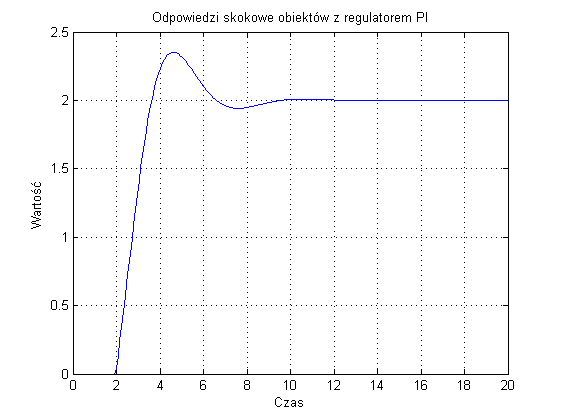
\includegraphics[scale=1]{images/jeden/skrypt_28.png}\\
\end{center}
\newpage
T = 10
\begin{center}
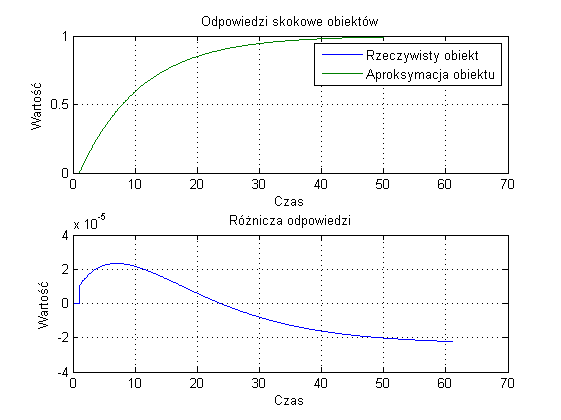
\includegraphics[scale=1]{images/jeden/skrypt_29.png}\\
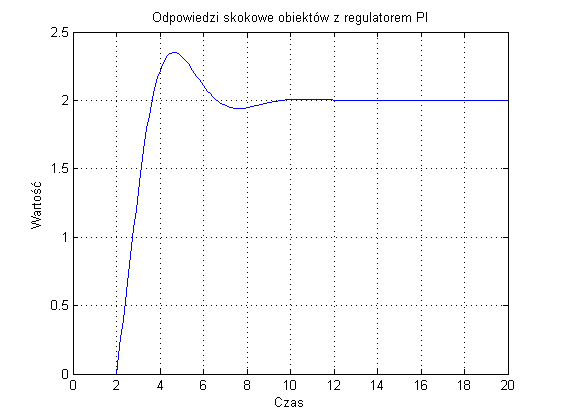
\includegraphics[scale=1]{images/jeden/skrypt_30.png}\\
\end{center}
\newpage
T = 20
\begin{center}
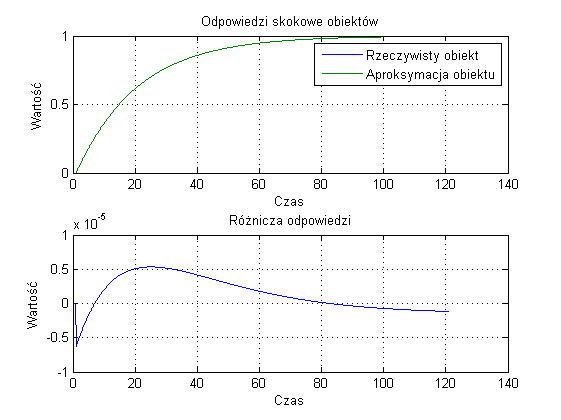
\includegraphics[scale=1]{images/jeden/skrypt_31.png}\\
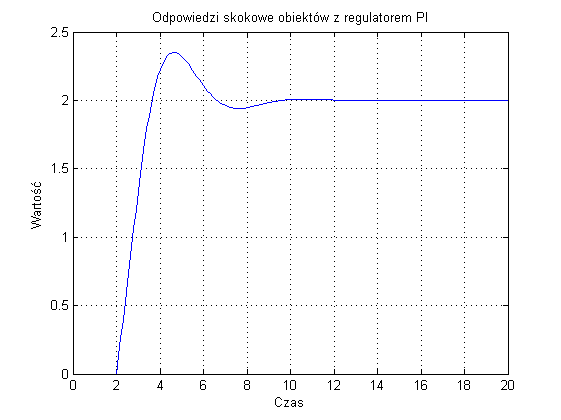
\includegraphics[scale=1]{images/jeden/skrypt_32.png}\\
\end{center}
\newpage
T = 50
\begin{center}
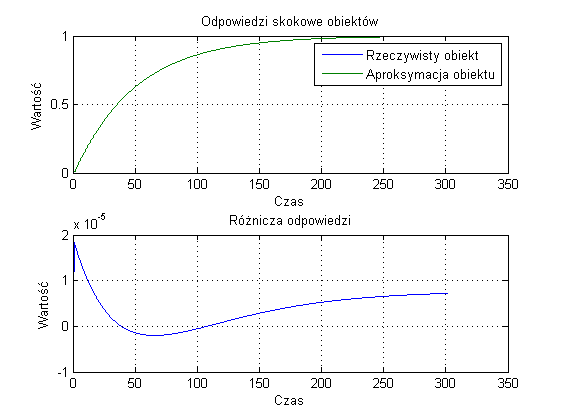
\includegraphics[scale=1]{images/jeden/skrypt_33.png}\\
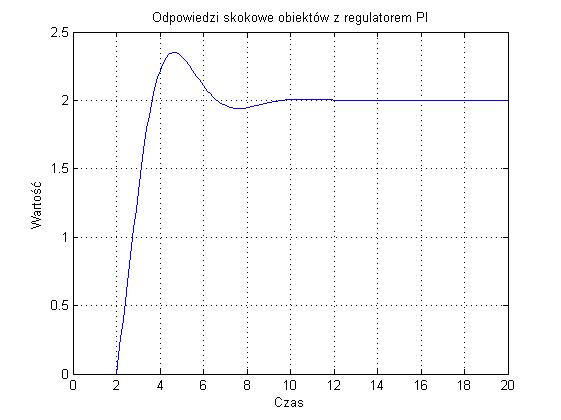
\includegraphics[scale=1]{images/jeden/skrypt_34.png}\\
\end{center}
\newpage
T = 100
\begin{center}
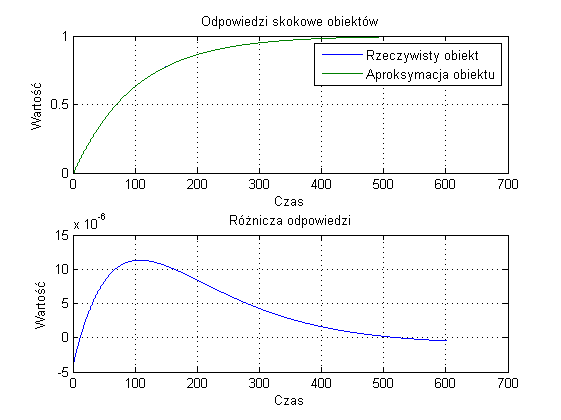
\includegraphics[scale=1]{images/jeden/skrypt_35.png}\\
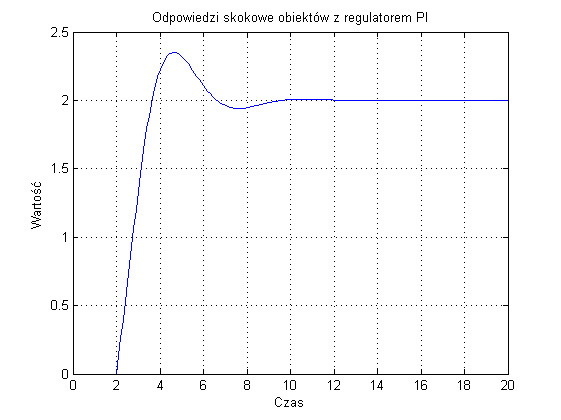
\includegraphics[scale=1]{images/jeden/skrypt_36.png}\\
\end{center}
\newpage
T = 200
\begin{center}
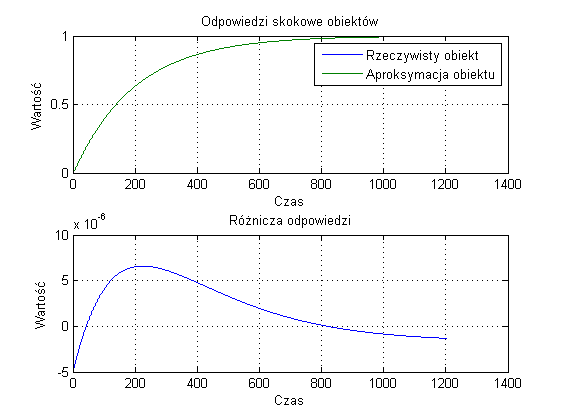
\includegraphics[scale=1]{images/jeden/skrypt_37.png}\\
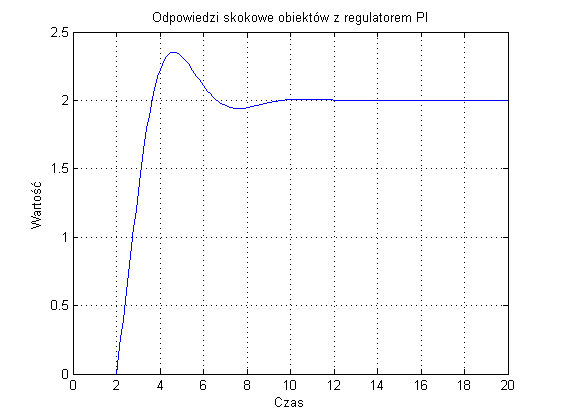
\includegraphics[scale=1]{images/jeden/skrypt_38.png}\\
\end{center}
\newpage
T = 500
\begin{center}
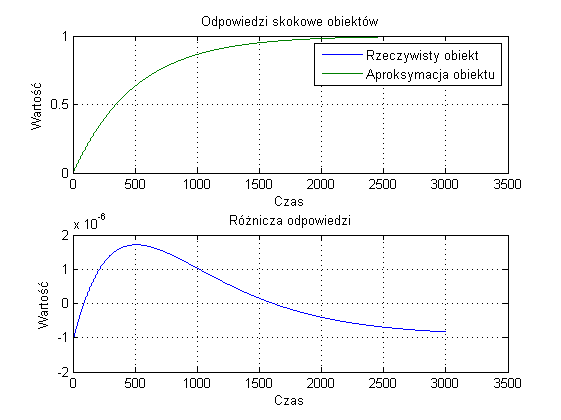
\includegraphics[scale=1]{images/jeden/skrypt_39.png}\\
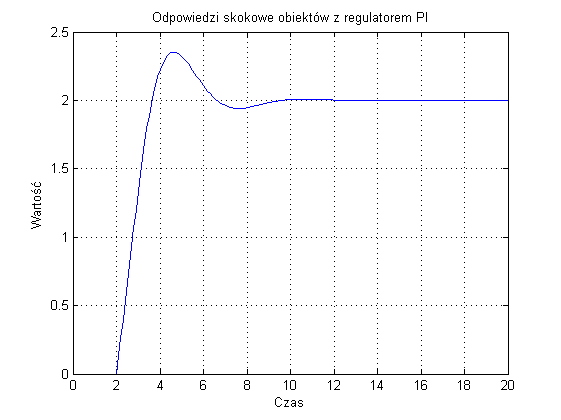
\includegraphics[scale=1]{images/jeden/skrypt_40.png}\\
\end{center}
\newpage
T = 1000
\begin{center}
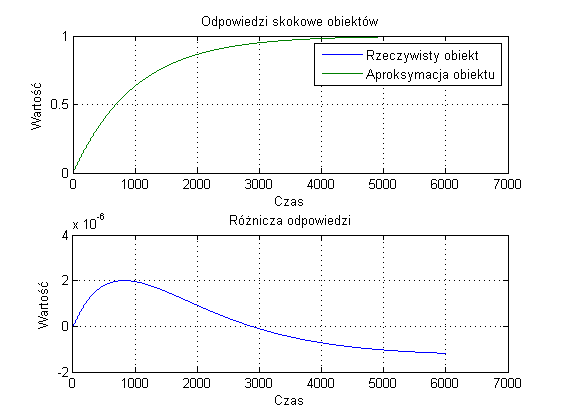
\includegraphics[scale=1]{images/jeden/skrypt_41.png}\\
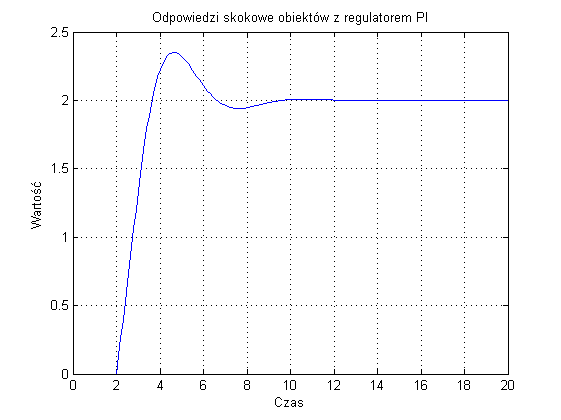
\includegraphics[scale=1]{images/jeden/skrypt_42.png}\\
\end{center}
\newpage

W pierwszym wypadku badanym obiektem był obiekt inercyjny I rzędu więc odpowiedzi skokowe aproksymacji są bardzo dokładne. Powyższe wykresy przedstawiające zachowania zamkniętych pętli z regulatorem PI pokazują, że nastawy regulatora dobrane metodą Haalman’a są bardzo dobre ponieważ stabilizują układ na wartości zadanej. Warto również zauważyć, że odpowiedzi dla każdej ze stałych czasowych są takie same. Spowodowane jest to faktem, że celem metody jest aby transmitancja zastępcza obiektu i regulatora była zależna jedynie od opóźnienia obiektu. Widać więc, że gdy uda nam się otrzymać bardzo dobry model obiektu sterowanego dynamika całego układu nie jest zależna od jego stałych czasowych. Widać wiec, że metoda jest bardzo przydatna kiedy chcemy sterować obiektami o bardzo dużych stałych czasowych. Niestety w odwrotnym przypadku gdy obiekt jest bardzo szybki nastawy regulatora dobrane naszą metodą mogą nie być zbyt efektowne gdy zależy nam na szybkim działaniu układu sterowania. 
\newpage
\subsection{Obiekt $P_2$}
T = 0.01
\begin{center}
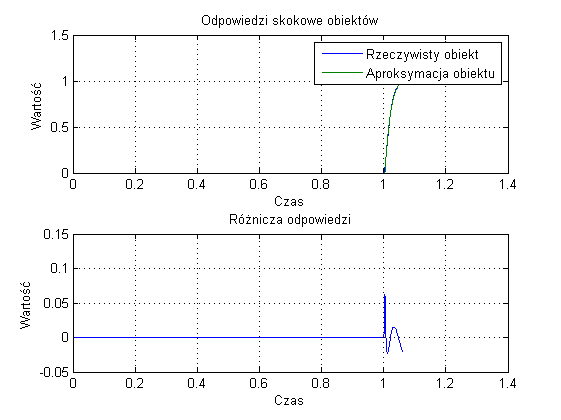
\includegraphics[scale=1]{images/jeden/skrypt_43.png}\\
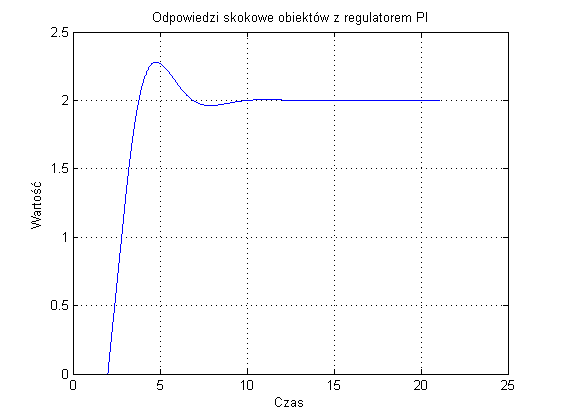
\includegraphics[scale=1]{images/jeden/skrypt_44.png}\\
\end{center}
\newpage
T = 0.02
\begin{center}
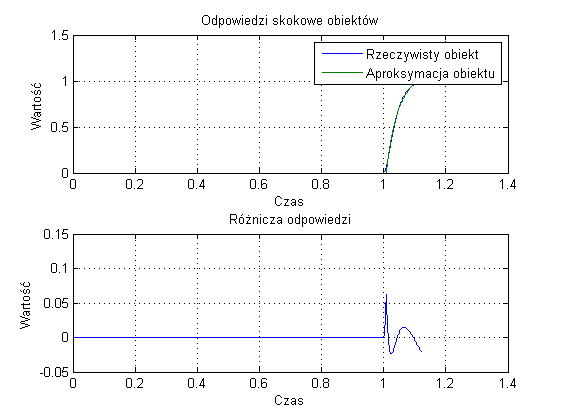
\includegraphics[scale=1]{images/jeden/skrypt_45.png}\\
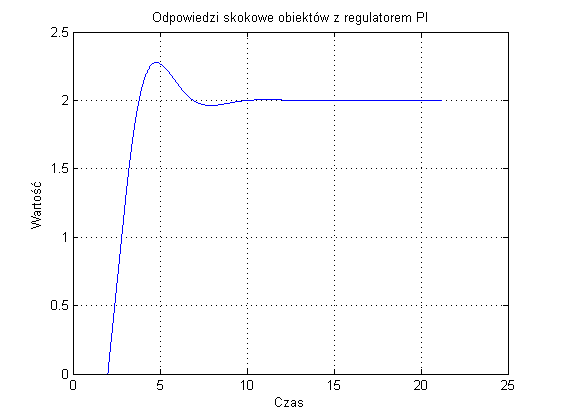
\includegraphics[scale=1]{images/jeden/skrypt_46.png}\\
\end{center}
\newpage
T = 0.05
\begin{center}
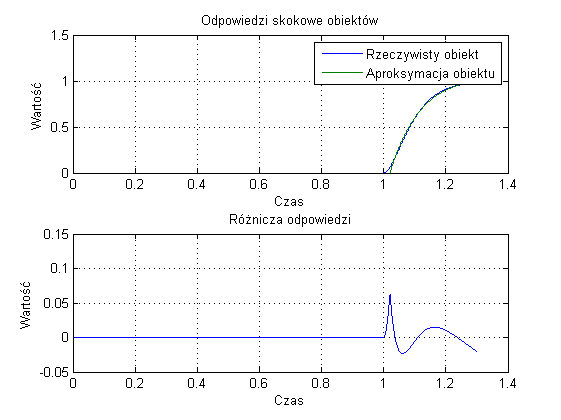
\includegraphics[scale=1]{images/jeden/skrypt_47.png}\\
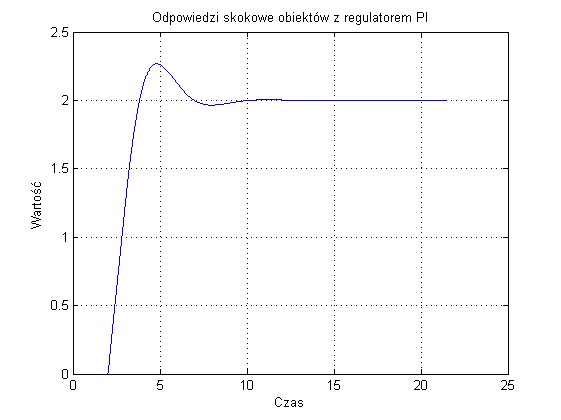
\includegraphics[scale=1]{images/jeden/skrypt_48.png}\\
\end{center}
\newpage
T = 0.1
\begin{center}
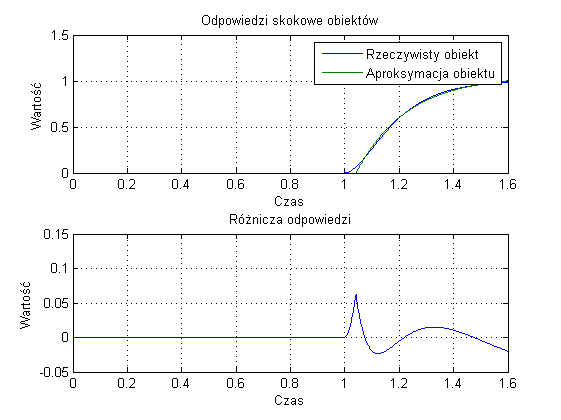
\includegraphics[scale=1]{images/jeden/skrypt_49.png}\\
\includegraphics[scale=1]{images/jeden/skrypt_50.png}\\
\end{center}
\newpage
T = 0.2
\begin{center}
\includegraphics[scale=1]{images/jeden/skrypt_51.png}\\
\includegraphics[scale=1]{images/jeden/skrypt_52.png}\\
\end{center}
\newpage
T = 0.3
\begin{center}
\includegraphics[scale=1]{images/jeden/skrypt_53.png}\\
\includegraphics[scale=1]{images/jeden/skrypt_54.png}\\
\end{center}
\newpage
T = 0.5
\begin{center}
\includegraphics[scale=1]{images/jeden/skrypt_55.png}\\
\includegraphics[scale=1]{images/jeden/skrypt_56.png}\\
\end{center}
\newpage
T = 0.7
\begin{center}
\includegraphics[scale=1]{images/jeden/skrypt_57.png}\\
\includegraphics[scale=1]{images/jeden/skrypt_58.png}\\
\end{center}
\newpage
T = 1
\begin{center}
\includegraphics[scale=1]{images/jeden/skrypt_59.png}\\
\includegraphics[scale=1]{images/jeden/skrypt_60.png}\\
\end{center}
\newpage
T = 1.3
\begin{center}
\includegraphics[scale=1]{images/jeden/skrypt_61.png}\\
\includegraphics[scale=1]{images/jeden/skrypt_62.png}\\
\end{center}
\newpage
T = 1.5
\begin{center}
\includegraphics[scale=1]{images/jeden/skrypt_63.png}\\
\includegraphics[scale=1]{images/jeden/skrypt_64.png}\\
\end{center}
\newpage
T = 2
\begin{center}
\includegraphics[scale=1]{images/jeden/skrypt_65.png}\\
\includegraphics[scale=1]{images/jeden/skrypt_66.png}\\
\end{center}
\newpage
T = 4
\begin{center}
\includegraphics[scale=1]{images/jeden/skrypt_67.png}\\
\includegraphics[scale=1]{images/jeden/skrypt_68.png}\\
\end{center}
\newpage
T = 6
\begin{center}
\includegraphics[scale=1]{images/jeden/skrypt_69.png}\\
\includegraphics[scale=1]{images/jeden/skrypt_70.png}\\
\end{center}
\newpage
T = 8
\begin{center}
\includegraphics[scale=1]{images/jeden/skrypt_71.png}\\
\includegraphics[scale=1]{images/jeden/skrypt_72.png}\\
\end{center}
\newpage
T = 10
\begin{center}
\includegraphics[scale=1]{images/jeden/skrypt_73.png}\\
\includegraphics[scale=1]{images/jeden/skrypt_74.png}\\
\end{center}
\newpage
T = 20
\begin{center}
\includegraphics[scale=1]{images/jeden/skrypt_75.png}\\
\includegraphics[scale=1]{images/jeden/skrypt_76.png}\\
\end{center}
\newpage
T = 50
\begin{center}
\includegraphics[scale=1]{images/jeden/skrypt_77.png}\\
\includegraphics[scale=1]{images/jeden/skrypt_78.png}\\
\end{center}
\newpage
T = 100
\begin{center}
\includegraphics[scale=1]{images/jeden/skrypt_79.png}\\
\includegraphics[scale=1]{images/jeden/skrypt_80.png}\\
\end{center}
\newpage
T = 200
\begin{center}
\includegraphics[scale=1]{images/jeden/skrypt_81.png}\\
\includegraphics[scale=1]{images/jeden/skrypt_82.png}\\
\end{center}
\newpage
T = 500
\begin{center}
\includegraphics[scale=1]{images/jeden/skrypt_83.png}\\
\includegraphics[scale=1]{images/jeden/skrypt_84.png}\\
\end{center}
\newpage
W drugim przypadku sterowanym obiektem był układ II rzędu o takich samych stałych czasowych. Układ regulacji również działa poprawnie stabilizując układ na wartości zadanej jednak wraz ze wzrostem stałej czasowej obiektu wzrasta czas potrzebny na jego stabilizacje oraz liczba przeregulowań. Spowodowane jest to faktem, że w transmitancji zastępczej układu znajduje się stała czasowa sterowanego obiektu niezniesiona przez regulator, która w znaczący sposób wpływa na dynamikę układu regulacji.
\newpage
\subsection{Obiekt $P_3$}
T = 0.005
\begin{center}
\includegraphics[scale=1]{images/jeden/skrypt_85.png}\\
\includegraphics[scale=1]{images/jeden/skrypt_86.png}\\
\end{center}
\newpage
T = 0.01
\begin{center}
\includegraphics[scale=1]{images/jeden/skrypt_87.png}\\
\includegraphics[scale=1]{images/jeden/skrypt_88.png}\\
\end{center}
\newpage
T = 0.02
\begin{center}
\includegraphics[scale=1]{images/jeden/skrypt_89.png}\\
\includegraphics[scale=1]{images/jeden/skrypt_90.png}\\
\end{center}
\newpage
T = 0.05
\begin{center}
\includegraphics[scale=1]{images/jeden/skrypt_91.png}\\
\includegraphics[scale=1]{images/jeden/skrypt_92.png}\\
\end{center}
\newpage
T = 0.1
\begin{center}
\includegraphics[scale=1]{images/jeden/skrypt_93.png}\\
\includegraphics[scale=1]{images/jeden/skrypt_94.png}\\
\end{center}
\newpage
T = 0.2
\begin{center}
\includegraphics[scale=1]{images/jeden/skrypt_95.png}\\
\includegraphics[scale=1]{images/jeden/skrypt_96.png}\\
\end{center}
\newpage
T = 0.5
\begin{center}
\includegraphics[scale=1]{images/jeden/skrypt_97.png}\\
\includegraphics[scale=1]{images/jeden/skrypt_98.png}\\
\end{center}
\newpage
T = 2
\begin{center}
\includegraphics[scale=1]{images/jeden/skrypt_99.png}\\
\includegraphics[scale=1]{images/jeden/skrypt_100.png}\\
\end{center}
\newpage
T = 5
\begin{center}
\includegraphics[scale=1]{images/jeden/skrypt_101.png}\\
\includegraphics[scale=1]{images/jeden/skrypt_102.png}\\
\end{center}
\newpage
T = 10
\begin{center}
\includegraphics[scale=1]{images/jeden/skrypt_103.png}\\
\includegraphics[scale=1]{images/jeden/skrypt_104.png}\\
\end{center}
\newpage
W trzecim przypadku mamy do czynienia z obiektem o stałej czasowej 1 oraz drugiej podwójnej. Również w tym przypadku regulator spełnia swoje zadanie sprowadzając układ do wartości zadanej. Jednak podobnie jak w drugim przypadku wraz ze wzrostem podwójnej stałej czasowej czas sterowania wydłuża się oraz zwiększa się ilość przeregulowań. Szczególnie widoczne jest to na wykresach dla trzech ostatnich stałych czasowych gdyż są one większe niż 1 i dlatego to one posiadają dominujący wpływ zarówno na dynamikę całego systemu jak i na parametry aproksymowanego obiektu I rzędu, który wyznacza parametry regulatora PI. 
\newpage
\subsection{Obiekt $P_4$}
n = 3
\begin{center}
\includegraphics[scale=1]{images/jeden/skrypt_105.png}\\
\includegraphics[scale=1]{images/jeden/skrypt_106.png}\\
\end{center}
\newpage
n = 4
\begin{center}
\includegraphics[scale=1]{images/jeden/skrypt_107.png}\\
\includegraphics[scale=1]{images/jeden/skrypt_108.png}\\
\end{center}
\newpage
n = 5
\begin{center}
\includegraphics[scale=1]{images/jeden/skrypt_109.png}\\
\includegraphics[scale=1]{images/jeden/skrypt_110.png}\\
\end{center}
\newpage
n = 6
\begin{center}
\includegraphics[scale=1]{images/jeden/skrypt_111.png}\\
\includegraphics[scale=1]{images/jeden/skrypt_112.png}\\
\end{center}
\newpage
n = 7
\begin{center}
\includegraphics[scale=1]{images/jeden/skrypt_113.png}\\
\includegraphics[scale=1]{images/jeden/skrypt_114.png}\\
\end{center}
\newpage
n = 8
\begin{center}
\includegraphics[scale=1]{images/jeden/skrypt_115.png}\\
\includegraphics[scale=1]{images/jeden/skrypt_116.png}\\
\end{center}
\newpage
W czwartym przypadku sterujemy obiektem, który posiada wielokrotną stałą czasową 1. Regulator sprowadza układ to zadanej wartości jednak wraz ze wzrostem stopnia mianownika transmitancji obiektu wrasta czas regulacji mimo, że błąd aproksymacji we wszystkich przypadkach jest podobny. Widać więc, że niezwalczone przez regulator bieguny obiektu są odpowiedzialne za zwiększający się czas regulacji.
\newpage
\subsection{Obiekt $P_5$}
$\alpha$ = 0.1
\begin{center}
\includegraphics[scale=1]{images/jeden/skrypt_117.png}\\
\includegraphics[scale=1]{images/jeden/skrypt_118.png}\\
\end{center}
\newpage
$\alpha$ = 0.2
\begin{center}
\includegraphics[scale=1]{images/jeden/skrypt_119.png}\\
\includegraphics[scale=1]{images/jeden/skrypt_120.png}\\
\end{center}
\newpage
$\alpha$ = 0.3
\begin{center}
\includegraphics[scale=1]{images/jeden/skrypt_121.png}\\
\includegraphics[scale=1]{images/jeden/skrypt_122.png}\\
\end{center}
\newpage
$\alpha$ = 0.4
\begin{center}
\includegraphics[scale=1]{images/jeden/skrypt_123.png}\\
\includegraphics[scale=1]{images/jeden/skrypt_124.png}\\
\end{center}
\newpage
$\alpha$ = 0.5
\begin{center}
\includegraphics[scale=1]{images/jeden/skrypt_125.png}\\
\includegraphics[scale=1]{images/jeden/skrypt_126.png}\\
\end{center}
\newpage
$\alpha$ = 0.6
\begin{center}
\includegraphics[scale=1]{images/jeden/skrypt_127.png}\\
\includegraphics[scale=1]{images/jeden/skrypt_128.png}\\
\end{center}
\newpage
$\alpha$ = 0.7
\begin{center}
\includegraphics[scale=1]{images/jeden/skrypt_129.png}\\
\includegraphics[scale=1]{images/jeden/skrypt_130.png}\\
\end{center}
\newpage
$\alpha$ = 0.8
\begin{center}
\includegraphics[scale=1]{images/jeden/skrypt_131.png}\\
\includegraphics[scale=1]{images/jeden/skrypt_132.png}\\
\end{center}
\newpage
$\alpha$ = 0.9
\begin{center}
\includegraphics[scale=1]{images/jeden/skrypt_133.png}\\
\includegraphics[scale=1]{images/jeden/skrypt_134.png}\\
\end{center}
\newpage
Zachowanie układu regulacji w piątym przypadku jest takie same jak w poprzednich symulacjach. Regulator stabilizuje układ na zadanej wartości jednak wraz ze wzrostem parametru $\alpha$ rośnie czas regulacji oraz przeregulowania. W piątym przypadku wpływ wzrostu jest bardziej widoczny ponieważ parametr $\alpha$ wpływa na trzy stałe czasowe obiektu.
\newpage
\subsection{Obiekt $P_6$}
$L_1$ = 0.01
\begin{center}
\includegraphics[scale=1]{images/jeden/skrypt_135.png}\\
\includegraphics[scale=1]{images/jeden/skrypt_136.png}\\
\end{center}
\newpage
$L_1$ = 0.02
\begin{center}
\includegraphics[scale=1]{images/jeden/skrypt_137.png}\\
\includegraphics[scale=1]{images/jeden/skrypt_138.png}\\
\end{center}
\newpage
$L_1$ = 0.05
\begin{center}
\includegraphics[scale=1]{images/jeden/skrypt_139.png}\\
\includegraphics[scale=1]{images/jeden/skrypt_140.png}\\
\end{center}
\newpage
$L_1$ = 0.1
\begin{center}
\includegraphics[scale=1]{images/jeden/skrypt_141.png}\\
\includegraphics[scale=1]{images/jeden/skrypt_142.png}\\
\end{center}
\newpage
$L_1$ = 0.3
\begin{center}
\includegraphics[scale=1]{images/jeden/skrypt_143.png}\\
\includegraphics[scale=1]{images/jeden/skrypt_144.png}\\
\end{center}
\newpage
$L_1$ = 0.5
\begin{center}
\includegraphics[scale=1]{images/jeden/skrypt_145.png}\\
\includegraphics[scale=1]{images/jeden/skrypt_146.png}\\
\end{center}
\newpage
$L_1$ = 0.7
\begin{center}
\includegraphics[scale=1]{images/jeden/skrypt_147.png}\\
\includegraphics[scale=1]{images/jeden/skrypt_148.png}\\
\end{center}
\newpage
$L_1$ = 0.8
\begin{center}
\includegraphics[scale=1]{images/jeden/skrypt_149.png}\\
\includegraphics[scale=1]{images/jeden/skrypt_150.png}\\
\end{center}
\newpage
$L_1$ = 0.9
\begin{center}
\includegraphics[scale=1]{images/jeden/skrypt_151.png}\\
\includegraphics[scale=1]{images/jeden/skrypt_152.png}\\
\end{center}
\newpage
W szóstym przypadku sterowany obiekt posiada człon całkujący co sprawia, że przybliżenie jego dynamiki obiektem inercyjnym I rzędu jest dokładne tylko na badanym odcinku czasowym. Mimo tego również i w tym przypadku regulator PI z nastawami dobranym metodą Haalman’a sprowadza układ do zadanej wartości w zadowalającym czasie. Zmiany parametrów obiektu sterowanego nie wpłynęły znacząco na dynamikę całego układu regulacji.
\newpage
\subsection{Obiekt $P_7$}
T = 1
$L_1$ = 0.01
\begin{center}
\includegraphics[scale=1]{images/jeden/skrypt_153.png}\\
\includegraphics[scale=1]{images/jeden/skrypt_154.png}\\
\end{center}
\newpage
$L_1$ = 0.02
\begin{center}
\includegraphics[scale=1]{images/jeden/skrypt_155.png}\\
\includegraphics[scale=1]{images/jeden/skrypt_156.png}\\
\end{center}
\newpage
$L_1$ = 0.05
\begin{center}
\includegraphics[scale=1]{images/jeden/skrypt_157.png}\\
\includegraphics[scale=1]{images/jeden/skrypt_158.png}\\
\end{center}
\newpage
$L_1$ = 0.1
\begin{center}
\includegraphics[scale=1]{images/jeden/skrypt_159.png}\\
\includegraphics[scale=1]{images/jeden/skrypt_160.png}\\
\end{center}
\newpage
$L_1$ = 0.3
\begin{center}
\includegraphics[scale=1]{images/jeden/skrypt_161.png}\\
\includegraphics[scale=1]{images/jeden/skrypt_162.png}\\
\end{center}
\newpage
$L_1$ = 0.5
\begin{center}
\includegraphics[scale=1]{images/jeden/skrypt_163.png}\\
\includegraphics[scale=1]{images/jeden/skrypt_164.png}\\
\end{center}
\newpage
$L_1$ = 0.7
\begin{center}
\includegraphics[scale=1]{images/jeden/skrypt_165.png}\\
\includegraphics[scale=1]{images/jeden/skrypt_166.png}\\
\end{center}
\newpage
$L_1$ = 0.8
\begin{center}
\includegraphics[scale=1]{images/jeden/skrypt_167.png}\\
\includegraphics[scale=1]{images/jeden/skrypt_168.png}\\
\end{center}
\newpage
$L_1$ = 0.9
\begin{center}
\includegraphics[scale=1]{images/jeden/skrypt_169.png}\\
\includegraphics[scale=1]{images/jeden/skrypt_170.png}\\
\end{center}
\newpage
T = 2
$L_1$ = 0.01
\begin{center}
\includegraphics[scale=1]{images/jeden/skrypt_171.png}\\
\includegraphics[scale=1]{images/jeden/skrypt_172.png}\\
\end{center}
\newpage
$L_1$ = 0.02
\begin{center}
\includegraphics[scale=1]{images/jeden/skrypt_173.png}\\
\includegraphics[scale=1]{images/jeden/skrypt_174.png}\\
\end{center}
\newpage
$L_1$ = 0.05
\begin{center}
\includegraphics[scale=1]{images/jeden/skrypt_175.png}\\
\includegraphics[scale=1]{images/jeden/skrypt_176.png}\\
\end{center}
\newpage
$L_1$ = 0.1
\begin{center}
\includegraphics[scale=1]{images/jeden/skrypt_177.png}\\
\includegraphics[scale=1]{images/jeden/skrypt_178.png}\\
\end{center}
\newpage
$L_1$ = 0.3
\begin{center}
\includegraphics[scale=1]{images/jeden/skrypt_179.png}\\
\includegraphics[scale=1]{images/jeden/skrypt_180.png}\\
\end{center}
\newpage
$L_1$ = 0.5
\begin{center}
\includegraphics[scale=1]{images/jeden/skrypt_181.png}\\
\includegraphics[scale=1]{images/jeden/skrypt_182.png}\\
\end{center}
\newpage
$L_1$ = 0.7
\begin{center}
\includegraphics[scale=1]{images/jeden/skrypt_183.png}\\
\includegraphics[scale=1]{images/jeden/skrypt_184.png}\\
\end{center}
\newpage
$L_1$ = 0.8
\begin{center}
\includegraphics[scale=1]{images/jeden/skrypt_185.png}\\
\includegraphics[scale=1]{images/jeden/skrypt_186.png}\\
\end{center}
\newpage
$L_1$ = 0.9
\begin{center}
\includegraphics[scale=1]{images/jeden/skrypt_187.png}\\
\includegraphics[scale=1]{images/jeden/skrypt_188.png}\\
\end{center}
\newpage
T = 5
$L_1$ = 0.01
\begin{center}
\includegraphics[scale=1]{images/jeden/skrypt_189.png}\\
\includegraphics[scale=1]{images/jeden/skrypt_190.png}\\
\end{center}
\newpage
$L_1$ = 0.02
\begin{center}
\includegraphics[scale=1]{images/jeden/skrypt_191.png}\\
\includegraphics[scale=1]{images/jeden/skrypt_192.png}\\
\end{center}
\newpage
$L_1$ = 0.05
\begin{center}
\includegraphics[scale=1]{images/jeden/skrypt_193.png}\\
\includegraphics[scale=1]{images/jeden/skrypt_194.png}\\
\end{center}
\newpage
$L_1$ = 0.1
\begin{center}
\includegraphics[scale=1]{images/jeden/skrypt_195.png}\\
\includegraphics[scale=1]{images/jeden/skrypt_196.png}\\
\end{center}
\newpage
$L_1$ = 0.3
\begin{center}
\includegraphics[scale=1]{images/jeden/skrypt_197.png}\\
\includegraphics[scale=1]{images/jeden/skrypt_198.png}\\
\end{center}
\newpage
$L_1$ = 0.5
\begin{center}
\includegraphics[scale=1]{images/jeden/skrypt_199.png}\\
\includegraphics[scale=1]{images/jeden/skrypt_200.png}\\
\end{center}
\newpage
$L_1$ = 0.7
\begin{center}
\includegraphics[scale=1]{images/jeden/skrypt_201.png}\\
\includegraphics[scale=1]{images/jeden/skrypt_202.png}\\
\end{center}
\newpage
$L_1$ = 0.8
\begin{center}
\includegraphics[scale=1]{images/jeden/skrypt_203.png}\\
\includegraphics[scale=1]{images/jeden/skrypt_204.png}\\
\end{center}
\newpage
$L_1$ = 0.9
\begin{center}
\includegraphics[scale=1]{images/jeden/skrypt_205.png}\\
\includegraphics[scale=1]{images/jeden/skrypt_206.png}\\
\end{center}
\newpage
T = 10
$L_1$ = 0.01
\begin{center}
\includegraphics[scale=1]{images/jeden/skrypt_207.png}\\
\includegraphics[scale=1]{images/jeden/skrypt_208.png}\\
\end{center}
\newpage
$L_1$ = 0.02
\begin{center}
\includegraphics[scale=1]{images/jeden/skrypt_209.png}\\
\includegraphics[scale=1]{images/jeden/skrypt_210.png}\\
\end{center}
\newpage
$L_1$ = 0.05
\begin{center}
\includegraphics[scale=1]{images/jeden/skrypt_211.png}\\
\includegraphics[scale=1]{images/jeden/skrypt_212.png}\\
\end{center}
\newpage
$L_1$ = 0.1
\begin{center}
\includegraphics[scale=1]{images/jeden/skrypt_213.png}\\
\includegraphics[scale=1]{images/jeden/skrypt_214.png}\\
\end{center}
\newpage
$L_1$ = 0.3
\begin{center}
\includegraphics[scale=1]{images/jeden/skrypt_215.png}\\
\includegraphics[scale=1]{images/jeden/skrypt_216.png}\\
\end{center}
\newpage
$L_1$ = 0.5
\begin{center}
\includegraphics[scale=1]{images/jeden/skrypt_217.png}\\
\includegraphics[scale=1]{images/jeden/skrypt_218.png}\\
\end{center}
\newpage
$L_1$ = 0.7
\begin{center}
\includegraphics[scale=1]{images/jeden/skrypt_219.png}\\
\includegraphics[scale=1]{images/jeden/skrypt_220.png}\\
\end{center}
\newpage
$L_1$ = 0.8
\begin{center}
\includegraphics[scale=1]{images/jeden/skrypt_221.png}\\
\includegraphics[scale=1]{images/jeden/skrypt_222.png}\\
\end{center}
\newpage
$L_1$ = 0.9
\begin{center}
\includegraphics[scale=1]{images/jeden/skrypt_223.png}\\
\includegraphics[scale=1]{images/jeden/skrypt_224.png}\\
\end{center}
\newpage
W siódmym przypadku regulator PI również radzi sobie bardzo dobrze z regulacją układu sprowadzając go do wartości zadanej. Widzimy także, że wraz ze wzrostem parametru L1, który powoduje spadek stałej czasowej T1 czas regulacji zmniejsza się ponieważ dynamika obiektu sterowanego coraz bardziej zbliża się do zachowań obiektu inercyjnego I rzędu co poprawia jakość regulacji ponieważ dla takiego typu obiektu stworzony jest docelowo regulator. Widać to było we wcześniejszych próbach gdy regulator PI najlepsze efekty dawał dla obiektu pierwszego czyli obiektu inercyjnego I rzędu.
\newpage
\subsection{Obiekt $P_8$}
$\alpha$ = 0.1
\begin{center}
\includegraphics[scale=1]{images/jeden/skrypt_225.png}\\
\includegraphics[scale=1]{images/jeden/skrypt_226.png}\\
\end{center}
\newpage
$\alpha$ = 0.2
\begin{center}
\includegraphics[scale=1]{images/jeden/skrypt_227.png}\\
\includegraphics[scale=1]{images/jeden/skrypt_228.png}\\
\end{center}
\newpage
$\alpha$ = 0.3
\begin{center}
\includegraphics[scale=1]{images/jeden/skrypt_229.png}\\
\includegraphics[scale=1]{images/jeden/skrypt_230.png}\\
\end{center}
\newpage
$\alpha$ = 0.4
\begin{center}
\includegraphics[scale=1]{images/jeden/skrypt_231.png}\\
\includegraphics[scale=1]{images/jeden/skrypt_232.png}\\
\end{center}
\newpage
$\alpha$ = 0.5
\begin{center}
\includegraphics[scale=1]{images/jeden/skrypt_233.png}\\
\includegraphics[scale=1]{images/jeden/skrypt_234.png}\\
\end{center}
\newpage
$\alpha$ = 0.6
\begin{center}
\includegraphics[scale=1]{images/jeden/skrypt_235.png}\\
\includegraphics[scale=1]{images/jeden/skrypt_236.png}\\
\end{center}
\newpage
$\alpha$ = 0.7
\begin{center}
\includegraphics[scale=1]{images/jeden/skrypt_237.png}\\
\includegraphics[scale=1]{images/jeden/skrypt_238.png}\\
\end{center}
\newpage
$\alpha$ = 0.8
\begin{center}
\includegraphics[scale=1]{images/jeden/skrypt_239.png}\\
\includegraphics[scale=1]{images/jeden/skrypt_240.png}\\
\end{center}
\newpage
$\alpha$ = 0.9
\begin{center}
\includegraphics[scale=1]{images/jeden/skrypt_241.png}\\
\includegraphics[scale=1]{images/jeden/skrypt_242.png}\\
\end{center}
\newpage
$\alpha$ = 1
\begin{center}
\includegraphics[scale=1]{images/jeden/skrypt_243.png}\\
\includegraphics[scale=1]{images/jeden/skrypt_244.png}\\
\end{center}
\newpage
$\alpha$ = 1.1
\begin{center}
\includegraphics[scale=1]{images/jeden/skrypt_245.png}\\
\includegraphics[scale=1]{images/jeden/skrypt_246.png}\\
\end{center}
\newpage
W przypadku obiektu minimalnofazowego układ po raz pierwszy nie działa tak dobrze jak w poprzednich przypadkach. Regulator stabilizuje układ jednak oscyluje on w bliskim otoczeniu wartości zadanej. Zmiana parametrów układu nie wpływa w żaden sposób na powstałe w układzie oscylacje.
\newpage
\subsection{Obiekt $P_9$}

T = 0.1
\begin{center}
\includegraphics[scale=1]{images/jeden/skrypt_247.png}\\
\includegraphics[scale=1]{images/jeden/skrypt_248.png}\\
\end{center}
\newpage
T = 0.2
\begin{center}
\includegraphics[scale=1]{images/jeden/skrypt_249.png}\\
\includegraphics[scale=1]{images/jeden/skrypt_250.png}\\
\end{center}
\newpage
T = 0.3
\begin{center}
\includegraphics[scale=1]{images/jeden/skrypt_251.png}\\
\includegraphics[scale=1]{images/jeden/skrypt_252.png}\\
\end{center}
\newpage
T = 0.4
\begin{center}
\includegraphics[scale=1]{images/jeden/skrypt_253.png}\\
\includegraphics[scale=1]{images/jeden/skrypt_254.png}\\
\end{center}
\newpage
T = 0.5
\begin{center}
\includegraphics[scale=1]{images/jeden/skrypt_255.png}\\
\includegraphics[scale=1]{images/jeden/skrypt_256.png}\\
\end{center}
\newpage
T = 0.6
\begin{center}
\includegraphics[scale=1]{images/jeden/skrypt_257.png}\\
\includegraphics[scale=1]{images/jeden/skrypt_258.png}\\
\end{center}
\newpage
T = 0.7
\begin{center}
\includegraphics[scale=1]{images/jeden/skrypt_259.png}\\
\includegraphics[scale=1]{images/jeden/skrypt_260.png}\\
\end{center}
\newpage
T = 0.8
\begin{center}
\includegraphics[scale=1]{images/jeden/skrypt_261.png}\\
\includegraphics[scale=1]{images/jeden/skrypt_262.png}\\
\end{center}
\newpage
T = 0.9
\begin{center}
\includegraphics[scale=1]{images/jeden/skrypt_263.png}\\
\includegraphics[scale=1]{images/jeden/skrypt_264.png}\\
\end{center}
\newpage
T = 1
\begin{center}
\includegraphics[scale=1]{images/jeden/skrypt_265.png}\\
\includegraphics[scale=1]{images/jeden/skrypt_266.png}\\
\end{center}
\newpage

W dziewiątym przypadku układ również stabilizuję się na wartości zadanej. Czas regulacji oraz przeregulowania również jak w poprzednich przypadkach rosną wraz ze wzrostem stałej czasowej układu.\\
Powyższe eksperymenty pokazały, że dobory nastaw regulatora PI metodą Haalman’a w zdecydowanej większości przypadków dają efekt w postaci stabilizacji układu. Widać także, że podczas wyliczania parametrów regulatora nie trzeba korzystać z skomplikowanej transmitancji obiektu sterowanego a można go przybliżyć obiektem inercyjnym I rzędu. Zauważyć również można, że gdy obiekt posiada duże stałe czasowe a nam zależy na szybkim czasie regulacji warto poszukać nastaw inną metodą. W przypadku szybkich obiektów efekty sterowania układy będą zadowalające.
\newpage

\section{Testy dla aproksymacji II rzędu}
Poniższe wykresy pokazują aproksymacje wszystkich obiektów obiektem inercyjnym II rzędu (na wykresach odpowiedź skokowa rzeczywistego obiektu oraz jego aproksymacji + błąd aproksymacji) oraz odpowiedzi zamkniętych układów regulacji dla wymuszenia równego 2(t) dla wszystkich stałych.\\
Parametry obiektów podobnie jak w przypadku obiektów I rzędu zostały wyznaczone przy pomocy funkcji fmincon().
\newpage
\subsection{Obiekt $P_1$}
T = 0.02
\begin{center}
\includegraphics[scale=1]{images/dwa/skrypt_01.png}\\
\includegraphics[scale=1]{images/dwa/skrypt_02.png}\\
\end{center}
\newpage
T = 0.05
\begin{center}
\includegraphics[scale=1]{images/dwa/skrypt_03.png}\\
\includegraphics[scale=1]{images/dwa/skrypt_04.png}\\
\end{center}
\newpage
T = 0.1
\begin{center}
\includegraphics[scale=1]{images/dwa/skrypt_05.png}\\
\includegraphics[scale=1]{images/dwa/skrypt_06.png}\\
\end{center}
\newpage
T = 0.2
\begin{center}
\includegraphics[scale=1]{images/dwa/skrypt_07.png}\\
\includegraphics[scale=1]{images/dwa/skrypt_08.png}\\
\end{center}
\newpage
T = 0.3
\begin{center}
\includegraphics[scale=1]{images/dwa/skrypt_09.png}\\
\includegraphics[scale=1]{images/dwa/skrypt_10.png}\\
\end{center}
\newpage
T = 0.5
\begin{center}
\includegraphics[scale=1]{images/dwa/skrypt_11.png}\\
\includegraphics[scale=1]{images/dwa/skrypt_12.png}\\
\end{center}
\newpage
T = 0.7
\begin{center}
\includegraphics[scale=1]{images/dwa/skrypt_13.png}\\
\includegraphics[scale=1]{images/dwa/skrypt_14.png}\\
\end{center}
\newpage
T = 1
\begin{center}
\includegraphics[scale=1]{images/dwa/skrypt_15.png}\\
\includegraphics[scale=1]{images/dwa/skrypt_16.png}\\
\end{center}
\newpage
T = 1.3
\begin{center}
\includegraphics[scale=1]{images/dwa/skrypt_17.png}\\
\includegraphics[scale=1]{images/dwa/skrypt_18.png}\\
\end{center}
\newpage
T = 1.5
\begin{center}
\includegraphics[scale=1]{images/dwa/skrypt_19.png}\\
\includegraphics[scale=1]{images/dwa/skrypt_20.png}\\
\end{center}
\newpage
T = 2
\begin{center}
\includegraphics[scale=1]{images/dwa/skrypt_21.png}\\
\includegraphics[scale=1]{images/dwa/skrypt_22.png}\\
\end{center}
\newpage
T = 4
\begin{center}
\includegraphics[scale=1]{images/dwa/skrypt_23.png}\\
\includegraphics[scale=1]{images/dwa/skrypt_24.png}\\
\end{center}
\newpage
T = 6
\begin{center}
\includegraphics[scale=1]{images/dwa/skrypt_25.png}\\
\includegraphics[scale=1]{images/dwa/skrypt_26.png}\\
\end{center}
\newpage
T = 8
\begin{center}
\includegraphics[scale=1]{images/dwa/skrypt_27.png}\\
\includegraphics[scale=1]{images/dwa/skrypt_28.png}\\
\end{center}
\newpage
T = 10
\begin{center}
\includegraphics[scale=1]{images/dwa/skrypt_29.png}\\
\includegraphics[scale=1]{images/dwa/skrypt_30.png}\\
\end{center}
\newpage
T = 20
\begin{center}
\includegraphics[scale=1]{images/dwa/skrypt_31.png}\\
\includegraphics[scale=1]{images/dwa/skrypt_32.png}\\
\end{center}
\newpage
T = 50
\begin{center}
\includegraphics[scale=1]{images/dwa/skrypt_33.png}\\
\includegraphics[scale=1]{images/dwa/skrypt_34.png}\\
\end{center}
\newpage
T = 100
\begin{center}
\includegraphics[scale=1]{images/dwa/skrypt_35.png}\\
\includegraphics[scale=1]{images/dwa/skrypt_36.png}\\
\end{center}
\newpage
T = 200
\begin{center}
\includegraphics[scale=1]{images/dwa/skrypt_37.png}\\
\includegraphics[scale=1]{images/dwa/skrypt_38.png}\\
\end{center}
\newpage
T = 500
\begin{center}
\includegraphics[scale=1]{images/dwa/skrypt_39.png}\\
\includegraphics[scale=1]{images/dwa/skrypt_40.png}\\
\end{center}
\newpage
T = 1000
\begin{center}
\includegraphics[scale=1]{images/dwa/skrypt_41.png}\\
\includegraphics[scale=1]{images/dwa/skrypt_42.png}\\
\end{center}
\newpage

W pierwszym przypadku gdy sterowanym obiektem był obiekt inercyjny I rzędu widać, że dla małych stałych czasowych regulator PID spełnia swoje zadanie. Jednak wraz ze wzrostem stałej T w układzie pojawiają się oscylacje. Spowodowane jest to tym znacznie rosnącą stałą $T_d$. Wzrost ten prowadzi do utraty stabilności przez układ więc widać, że lepszy efekt przyniósł regulator PI. 
 
\newpage
\subsection{Obiekt $P_2$}
T = 0.01
\begin{center}
\includegraphics[scale=1]{images/dwa/skrypt_43.png}\\
\includegraphics[scale=1]{images/dwa/skrypt_44.png}\\
\end{center}
\newpage
T = 0.02
\begin{center}
\includegraphics[scale=1]{images/dwa/skrypt_45.png}\\
\includegraphics[scale=1]{images/dwa/skrypt_46.png}\\
\end{center}
\newpage
T = 0.05
\begin{center}
\includegraphics[scale=1]{images/dwa/skrypt_47.png}\\
\includegraphics[scale=1]{images/dwa/skrypt_48.png}\\
\end{center}
\newpage
T = 0.1
\begin{center}
\includegraphics[scale=1]{images/dwa/skrypt_49.png}\\
\includegraphics[scale=1]{images/dwa/skrypt_50.png}\\
\end{center}
\newpage
T = 0.2
\begin{center}
\includegraphics[scale=1]{images/dwa/skrypt_51.png}\\
\includegraphics[scale=1]{images/dwa/skrypt_52.png}\\
\end{center}
\newpage
T = 0.3
\begin{center}
\includegraphics[scale=1]{images/dwa/skrypt_53.png}\\
\includegraphics[scale=1]{images/dwa/skrypt_54.png}\\
\end{center}
\newpage
T = 0.5
\begin{center}
\includegraphics[scale=1]{images/dwa/skrypt_55.png}\\
\includegraphics[scale=1]{images/dwa/skrypt_56.png}\\
\end{center}
\newpage
T = 0.7
\begin{center}
\includegraphics[scale=1]{images/dwa/skrypt_57.png}\\
\includegraphics[scale=1]{images/dwa/skrypt_58.png}\\
\end{center}
\newpage
T = 1
\begin{center}
\includegraphics[scale=1]{images/dwa/skrypt_59.png}\\
\includegraphics[scale=1]{images/dwa/skrypt_60.png}\\
\end{center}
\newpage
T = 1.3
\begin{center}
\includegraphics[scale=1]{images/dwa/skrypt_61.png}\\
\includegraphics[scale=1]{images/dwa/skrypt_62.png}\\
\end{center}
\newpage
T = 1.5
\begin{center}
\includegraphics[scale=1]{images/dwa/skrypt_63.png}\\
\includegraphics[scale=1]{images/dwa/skrypt_64.png}\\
\end{center}
\newpage
T = 2
\begin{center}
\includegraphics[scale=1]{images/dwa/skrypt_65.png}\\
\includegraphics[scale=1]{images/dwa/skrypt_66.png}\\
\end{center}
\newpage
T = 4
\begin{center}
\includegraphics[scale=1]{images/dwa/skrypt_67.png}\\
\includegraphics[scale=1]{images/dwa/skrypt_68.png}\\
\end{center}
\newpage
T = 6
\begin{center}
\includegraphics[scale=1]{images/dwa/skrypt_69.png}\\
\includegraphics[scale=1]{images/dwa/skrypt_70.png}\\
\end{center}
\newpage
T = 8
\begin{center}
\includegraphics[scale=1]{images/dwa/skrypt_71.png}\\
\includegraphics[scale=1]{images/dwa/skrypt_72.png}\\
\end{center}
\newpage
T = 10
\begin{center}
\includegraphics[scale=1]{images/dwa/skrypt_73.png}\\
\includegraphics[scale=1]{images/dwa/skrypt_74.png}\\
\end{center}
\newpage
T = 20
\begin{center}
\includegraphics[scale=1]{images/dwa/skrypt_75.png}\\
\includegraphics[scale=1]{images/dwa/skrypt_76.png}\\
\end{center}
\newpage
T = 50
\begin{center}
\includegraphics[scale=1]{images/dwa/skrypt_77.png}\\
\includegraphics[scale=1]{images/dwa/skrypt_78.png}\\
\end{center}
\newpage
T = 100
\begin{center}
\includegraphics[scale=1]{images/dwa/skrypt_79.png}\\
\includegraphics[scale=1]{images/dwa/skrypt_80.png}\\
\end{center}
\newpage
T = 200
\begin{center}
\includegraphics[scale=1]{images/dwa/skrypt_81.png}\\
\includegraphics[scale=1]{images/dwa/skrypt_82.png}\\
\end{center}
\newpage
T = 500
\begin{center}
\includegraphics[scale=1]{images/dwa/skrypt_83.png}\\
\includegraphics[scale=1]{images/dwa/skrypt_84.png}\\
\end{center}
\newpage
W drugim przypadku sterowanym obiektem był układ II rzędu o takich samych stałych czasowych. Układ regulacji również jak w przypadku z regulatorem PI działa poprawnie i stabilizuje układ na zadanej wartości. Niestety również tutaj mimo że regulator PID dobrany jest dokładnie dla obiektu inercyjnego II rzędu pojawiają się oscylacje wraz ze wzrostem stałej T jednak układ nie staje się niestabilny.
\newpage
\subsection{Obiekt $P_3$}
T = 0.005
\begin{center}
\includegraphics[scale=1]{images/dwa/skrypt_85.png}\\
\includegraphics[scale=1]{images/dwa/skrypt_86.png}\\
\end{center}
\newpage
T = 0.01
\begin{center}
\includegraphics[scale=1]{images/dwa/skrypt_87.png}\\
\includegraphics[scale=1]{images/dwa/skrypt_88.png}\\
\end{center}
\newpage
T = 0.02
\begin{center}
\includegraphics[scale=1]{images/dwa/skrypt_89.png}\\
\includegraphics[scale=1]{images/dwa/skrypt_90.png}\\
\end{center}
\newpage
T = 0.05
\begin{center}
\includegraphics[scale=1]{images/dwa/skrypt_91.png}\\
\includegraphics[scale=1]{images/dwa/skrypt_92.png}\\
\end{center}
\newpage
T = 0.1
\begin{center}
\includegraphics[scale=1]{images/dwa/skrypt_93.png}\\
\includegraphics[scale=1]{images/dwa/skrypt_94.png}\\
\end{center}
\newpage
T = 0.2
\begin{center}
\includegraphics[scale=1]{images/dwa/skrypt_95.png}\\
\includegraphics[scale=1]{images/dwa/skrypt_96.png}\\
\end{center}
\newpage
T = 0.5
\begin{center}
\includegraphics[scale=1]{images/dwa/skrypt_97.png}\\
\includegraphics[scale=1]{images/dwa/skrypt_98.png}\\
\end{center}
\newpage
T = 2
\begin{center}
\includegraphics[scale=1]{images/dwa/skrypt_99.png}\\
\includegraphics[scale=1]{images/dwa/skrypt_100.png}\\
\end{center}
\newpage
T = 5
\begin{center}
\includegraphics[scale=1]{images/dwa/skrypt_101.png}\\
\includegraphics[scale=1]{images/dwa/skrypt_102.png}\\
\end{center}
\newpage
T = 10
\begin{center}
\includegraphics[scale=1]{images/dwa/skrypt_103.png}\\
\includegraphics[scale=1]{images/dwa/skrypt_104.png}\\
\end{center}
\newpage
W trzecim przypadku mamy do czynienia z obiektem o stałej czasowej 1 oraz drugiej podwójnej. W tym przypadku nie ma silnego powiązania co do poprawności działania układu ze wzrostem parametru T. Widzimy, że dla pewnych stałych układ staje się nie stabilny a więc lepiej spisuje się dobrany regulator PI.
\newpage
\subsection{Obiekt $P_4$}
n = 3
\begin{center}
\includegraphics[scale=1]{images/dwa/skrypt_105.png}\\
\includegraphics[scale=1]{images/dwa/skrypt_106.png}\\
\end{center}
\newpage
n = 4
\begin{center}
\includegraphics[scale=1]{images/dwa/skrypt_107.png}\\
\includegraphics[scale=1]{images/dwa/skrypt_108.png}\\
\end{center}
\newpage
n = 5
\begin{center}
\includegraphics[scale=1]{images/dwa/skrypt_109.png}\\
\includegraphics[scale=1]{images/dwa/skrypt_110.png}\\
\end{center}
\newpage
n = 6
\begin{center}
\includegraphics[scale=1]{images/dwa/skrypt_111.png}\\
\includegraphics[scale=1]{images/dwa/skrypt_112.png}\\
\end{center}
\newpage
n = 7
\begin{center}
\includegraphics[scale=1]{images/dwa/skrypt_113.png}\\
\includegraphics[scale=1]{images/dwa/skrypt_114.png}\\
\end{center}
\newpage
n = 8
\begin{center}
\includegraphics[scale=1]{images/dwa/skrypt_115.png}\\
\includegraphics[scale=1]{images/dwa/skrypt_116.png}\\
\end{center}
\newpage
W czwartym przypadku sterujemy obiektem, który posiada wielokrotną stałą czasową 1. Regulator nie sprowadza układ to zadanej wartości tylko oscyluje w jej otoczeniu. Wraz ze wzrostem stopnia mianownika transmitancji obiektu zmniejsza się wielkość początkowych oscylacji ale zwiększa czas regulacji. Dla tego przypadku również lepiej spisał się regulator PI.
\newpage
\subsection{Obiekt $P_5$}
$\alpha$ = 0.1
\begin{center}
\includegraphics[scale=1]{images/dwa/skrypt_117.png}\\
\includegraphics[scale=1]{images/dwa/skrypt_118.png}\\
\end{center}
\newpage
$\alpha$ = 0.2
\begin{center}
\includegraphics[scale=1]{images/dwa/skrypt_119.png}\\
\includegraphics[scale=1]{images/dwa/skrypt_120.png}\\
\end{center}
\newpage
$\alpha$ = 0.3
\begin{center}
\includegraphics[scale=1]{images/dwa/skrypt_121.png}\\
\includegraphics[scale=1]{images/dwa/skrypt_122.png}\\
\end{center}
\newpage
$\alpha$ = 0.4
\begin{center}
\includegraphics[scale=1]{images/dwa/skrypt_123.png}\\
\includegraphics[scale=1]{images/dwa/skrypt_124.png}\\
\end{center}
\newpage
$\alpha$ = 0.5
\begin{center}
\includegraphics[scale=1]{images/dwa/skrypt_125.png}\\
\includegraphics[scale=1]{images/dwa/skrypt_126.png}\\
\end{center}
\newpage
$\alpha$ = 0.6
\begin{center}
\includegraphics[scale=1]{images/dwa/skrypt_127.png}\\
\includegraphics[scale=1]{images/dwa/skrypt_128.png}\\
\end{center}
\newpage
$\alpha$ = 0.7
\begin{center}
\includegraphics[scale=1]{images/dwa/skrypt_129.png}\\
\includegraphics[scale=1]{images/dwa/skrypt_130.png}\\
\end{center}
\newpage
$\alpha$ = 0.8
\begin{center}
\includegraphics[scale=1]{images/dwa/skrypt_131.png}\\
\includegraphics[scale=1]{images/dwa/skrypt_132.png}\\
\end{center}
\newpage
$\alpha$ = 0.9
\begin{center}
\includegraphics[scale=1]{images/dwa/skrypt_133.png}\\
\includegraphics[scale=1]{images/dwa/skrypt_134.png}\\
\end{center}
\newpage
Podczas symulacji piątego przypadku widać, że regulator spełnia swoje zadanie stabilizując układ na wartości zadanej. Wraz ze wzrostem parametru $\alpha$ wielkość przeregulowań maleje oraz zmniejsza się czas regulacji. Widać wiec, że dla tego typu układów z dużą stałą czasową lepiej zastosować regulator PID.
\newpage
\subsection{Obiekt $P_6$}
$L_1$ = 0.01
\begin{center}
\includegraphics[scale=1]{images/dwa/skrypt_135.png}\\
\includegraphics[scale=1]{images/dwa/skrypt_136.png}\\
\end{center}
\newpage
$L_1$ = 0.02
\begin{center}
\includegraphics[scale=1]{images/dwa/skrypt_137.png}\\
\includegraphics[scale=1]{images/dwa/skrypt_138.png}\\
\end{center}
\newpage
$L_1$ = 0.05
\begin{center}
\includegraphics[scale=1]{images/dwa/skrypt_139.png}\\
\includegraphics[scale=1]{images/dwa/skrypt_140.png}\\
\end{center}
\newpage
$L_1$ = 0.1
\begin{center}
\includegraphics[scale=1]{images/dwa/skrypt_141.png}\\
\includegraphics[scale=1]{images/dwa/skrypt_142.png}\\
\end{center}
\newpage
$L_1$ = 0.3
\begin{center}
\includegraphics[scale=1]{images/dwa/skrypt_143.png}\\
\includegraphics[scale=1]{images/dwa/skrypt_144.png}\\
\end{center}
\newpage
$L_1$ = 0.5
\begin{center}
\includegraphics[scale=1]{images/dwa/skrypt_145.png}\\
\includegraphics[scale=1]{images/dwa/skrypt_146.png}\\
\end{center}
\newpage
$L_1$ = 0.7
\begin{center}
\includegraphics[scale=1]{images/dwa/skrypt_147.png}\\
\includegraphics[scale=1]{images/dwa/skrypt_148.png}\\
\end{center}
\newpage
$L_1$ = 0.8
\begin{center}
\includegraphics[scale=1]{images/dwa/skrypt_149.png}\\
\includegraphics[scale=1]{images/dwa/skrypt_150.png}\\
\end{center}
\newpage
$L_1$ = 0.9
\begin{center}
\includegraphics[scale=1]{images/dwa/skrypt_151.png}\\
\includegraphics[scale=1]{images/dwa/skrypt_152.png}\\
\end{center}
\newpage
W szóstym przypadku regulator PID kompletnie się nie sprawdza sprawiając, że w większości przypadków układ staje się niestabilny. Dla obiektu z całkowaniem dużo bardziej sprawdza się regulator PI.
\newpage
\subsection{Obiekt $P_7$}
T = 1
$L_1$ = 0.01
\begin{center}
\includegraphics[scale=1]{images/dwa/skrypt_153.png}\\
\includegraphics[scale=1]{images/dwa/skrypt_154.png}\\
\end{center}
\newpage
$L_1$ = 0.02
\begin{center}
\includegraphics[scale=1]{images/dwa/skrypt_155.png}\\
\includegraphics[scale=1]{images/dwa/skrypt_156.png}\\
\end{center}
\newpage
$L_1$ = 0.05
\begin{center}
\includegraphics[scale=1]{images/dwa/skrypt_157.png}\\
\includegraphics[scale=1]{images/dwa/skrypt_158.png}\\
\end{center}
\newpage
$L_1$ = 0.1
\begin{center}
\includegraphics[scale=1]{images/dwa/skrypt_159.png}\\
\includegraphics[scale=1]{images/dwa/skrypt_160.png}\\
\end{center}
\newpage
$L_1$ = 0.3
\begin{center}
\includegraphics[scale=1]{images/dwa/skrypt_161.png}\\
\includegraphics[scale=1]{images/dwa/skrypt_162.png}\\
\end{center}
\newpage
$L_1$ = 0.5
\begin{center}
\includegraphics[scale=1]{images/dwa/skrypt_163.png}\\
\includegraphics[scale=1]{images/dwa/skrypt_164.png}\\
\end{center}
\newpage
$L_1$ = 0.7
\begin{center}
\includegraphics[scale=1]{images/dwa/skrypt_165.png}\\
\includegraphics[scale=1]{images/dwa/skrypt_166.png}\\
\end{center}
\newpage
$L_1$ = 0.8
\begin{center}
\includegraphics[scale=1]{images/dwa/skrypt_167.png}\\
\includegraphics[scale=1]{images/dwa/skrypt_168.png}\\
\end{center}
\newpage
$L_1$ = 0.9
\begin{center}
\includegraphics[scale=1]{images/dwa/skrypt_169.png}\\
\includegraphics[scale=1]{images/dwa/skrypt_170.png}\\
\end{center}
\newpage
T = 2
$L_1$ = 0.01
\begin{center}
\includegraphics[scale=1]{images/dwa/skrypt_171.png}\\
\includegraphics[scale=1]{images/dwa/skrypt_172.png}\\
\end{center}
\newpage
$L_1$ = 0.02
\begin{center}
\includegraphics[scale=1]{images/dwa/skrypt_173.png}\\
\includegraphics[scale=1]{images/dwa/skrypt_174.png}\\
\end{center}
\newpage
$L_1$ = 0.05
\begin{center}
\includegraphics[scale=1]{images/dwa/skrypt_175.png}\\
\includegraphics[scale=1]{images/dwa/skrypt_176.png}\\
\end{center}
\newpage
$L_1$ = 0.1
\begin{center}
\includegraphics[scale=1]{images/dwa/skrypt_177.png}\\
\includegraphics[scale=1]{images/dwa/skrypt_178.png}\\
\end{center}
\newpage
$L_1$ = 0.3
\begin{center}
\includegraphics[scale=1]{images/dwa/skrypt_179.png}\\
\includegraphics[scale=1]{images/dwa/skrypt_180.png}\\
\end{center}
\newpage
$L_1$ = 0.5
\begin{center}
\includegraphics[scale=1]{images/dwa/skrypt_181.png}\\
\includegraphics[scale=1]{images/dwa/skrypt_182.png}\\
\end{center}
\newpage
$L_1$ = 0.7
\begin{center}
\includegraphics[scale=1]{images/dwa/skrypt_183.png}\\
\includegraphics[scale=1]{images/dwa/skrypt_184.png}\\
\end{center}
\newpage
$L_1$ = 0.8
\begin{center}
\includegraphics[scale=1]{images/dwa/skrypt_185.png}\\
\includegraphics[scale=1]{images/dwa/skrypt_186.png}\\
\end{center}
\newpage
$L_1$ = 0.9
\begin{center}
\includegraphics[scale=1]{images/dwa/skrypt_187.png}\\
\includegraphics[scale=1]{images/dwa/skrypt_188.png}\\
\end{center}
\newpage
T = 5
$L_1$ = 0.01
\begin{center}
\includegraphics[scale=1]{images/dwa/skrypt_189.png}\\
\includegraphics[scale=1]{images/dwa/skrypt_190.png}\\
\end{center}
\newpage
$L_1$ = 0.02
\begin{center}
\includegraphics[scale=1]{images/dwa/skrypt_191.png}\\
\includegraphics[scale=1]{images/dwa/skrypt_192.png}\\
\end{center}
\newpage
$L_1$ = 0.05
\begin{center}
\includegraphics[scale=1]{images/dwa/skrypt_193.png}\\
\includegraphics[scale=1]{images/dwa/skrypt_194.png}\\
\end{center}
\newpage
$L_1$ = 0.1
\begin{center}
\includegraphics[scale=1]{images/dwa/skrypt_195.png}\\
\includegraphics[scale=1]{images/dwa/skrypt_196.png}\\
\end{center}
\newpage
$L_1$ = 0.3
\begin{center}
\includegraphics[scale=1]{images/dwa/skrypt_197.png}\\
\includegraphics[scale=1]{images/dwa/skrypt_198.png}\\
\end{center}
\newpage
$L_1$ = 0.5
\begin{center}
\includegraphics[scale=1]{images/dwa/skrypt_199.png}\\
\includegraphics[scale=1]{images/dwa/skrypt_200.png}\\
\end{center}
\newpage
$L_1$ = 0.7
\begin{center}
\includegraphics[scale=1]{images/dwa/skrypt_201.png}\\
\includegraphics[scale=1]{images/dwa/skrypt_202.png}\\
\end{center}
\newpage
$L_1$ = 0.8
\begin{center}
\includegraphics[scale=1]{images/dwa/skrypt_203.png}\\
\includegraphics[scale=1]{images/dwa/skrypt_204.png}\\
\end{center}
\newpage
$L_1$ = 0.9
\begin{center}
\includegraphics[scale=1]{images/dwa/skrypt_205.png}\\
\includegraphics[scale=1]{images/dwa/skrypt_206.png}\\
\end{center}
\newpage
T = 10
$L_1$ = 0.01
\begin{center}
\includegraphics[scale=1]{images/dwa/skrypt_207.png}\\
\includegraphics[scale=1]{images/dwa/skrypt_208.png}\\
\end{center}
\newpage
$L_1$ = 0.02
\begin{center}
\includegraphics[scale=1]{images/dwa/skrypt_209.png}\\
\includegraphics[scale=1]{images/dwa/skrypt_210.png}\\
\end{center}
\newpage
$L_1$ = 0.05
\begin{center}
\includegraphics[scale=1]{images/dwa/skrypt_211.png}\\
\includegraphics[scale=1]{images/dwa/skrypt_212.png}\\
\end{center}
\newpage
$L_1$ = 0.1
\begin{center}
\includegraphics[scale=1]{images/dwa/skrypt_213.png}\\
\includegraphics[scale=1]{images/dwa/skrypt_214.png}\\
\end{center}
\newpage
$L_1$ = 0.3
\begin{center}
\includegraphics[scale=1]{images/dwa/skrypt_215.png}\\
\includegraphics[scale=1]{images/dwa/skrypt_216.png}\\
\end{center}
\newpage
$L_1$ = 0.5
\begin{center}
\includegraphics[scale=1]{images/dwa/skrypt_217.png}\\
\includegraphics[scale=1]{images/dwa/skrypt_218.png}\\
\end{center}
\newpage
$L_1$ = 0.7
\begin{center}
\includegraphics[scale=1]{images/dwa/skrypt_219.png}\\
\includegraphics[scale=1]{images/dwa/skrypt_220.png}\\
\end{center}
\newpage
$L_1$ = 0.8
\begin{center}
\includegraphics[scale=1]{images/dwa/skrypt_221.png}\\
\includegraphics[scale=1]{images/dwa/skrypt_222.png}\\
\end{center}
\newpage
$L_1$ = 0.9
\begin{center}
\includegraphics[scale=1]{images/dwa/skrypt_223.png}\\
\includegraphics[scale=1]{images/dwa/skrypt_224.png}\\
\end{center}
\newpage
W siódmym przypadku regulator PID po raz kolejny nie radzi sobie ze sterowaniem układu znowu sprawiając, że staje się on niestabilny.
\newpage
\subsection{Obiekt $P_8$}
$\alpha$ = 0.1
\begin{center}
\includegraphics[scale=1]{images/dwa/skrypt_225.png}\\
\includegraphics[scale=1]{images/dwa/skrypt_226.png}\\
\end{center}
\newpage
$\alpha$ = 0.2
\begin{center}
\includegraphics[scale=1]{images/dwa/skrypt_227.png}\\
\includegraphics[scale=1]{images/dwa/skrypt_228.png}\\
\end{center}
\newpage
$\alpha$ = 0.3
\begin{center}
\includegraphics[scale=1]{images/dwa/skrypt_229.png}\\
\includegraphics[scale=1]{images/dwa/skrypt_230.png}\\
\end{center}
\newpage
$\alpha$ = 0.4
\begin{center}
\includegraphics[scale=1]{images/dwa/skrypt_231.png}\\
\includegraphics[scale=1]{images/dwa/skrypt_232.png}\\
\end{center}
\newpage
$\alpha$ = 0.5
\begin{center}
\includegraphics[scale=1]{images/dwa/skrypt_233.png}\\
\includegraphics[scale=1]{images/dwa/skrypt_234.png}\\
\end{center}
\newpage
$\alpha$ = 0.6
\begin{center}
\includegraphics[scale=1]{images/dwa/skrypt_235.png}\\
\includegraphics[scale=1]{images/dwa/skrypt_236.png}\\
\end{center}
\newpage
$\alpha$ = 0.7
\begin{center}
\includegraphics[scale=1]{images/dwa/skrypt_237.png}\\
\includegraphics[scale=1]{images/dwa/skrypt_238.png}\\
\end{center}
\newpage
$\alpha$ = 0.8
\begin{center}
\includegraphics[scale=1]{images/dwa/skrypt_239.png}\\
\includegraphics[scale=1]{images/dwa/skrypt_240.png}\\
\end{center}
\newpage
$\alpha$ = 0.9
\begin{center}
\includegraphics[scale=1]{images/dwa/skrypt_241.png}\\
\includegraphics[scale=1]{images/dwa/skrypt_242.png}\\
\end{center}
\newpage
$\alpha$ = 1
\begin{center}
\includegraphics[scale=1]{images/dwa/skrypt_243.png}\\
\includegraphics[scale=1]{images/dwa/skrypt_244.png}\\
\end{center}
\newpage
$\alpha$ = 1.1
\begin{center}
\includegraphics[scale=1]{images/dwa/skrypt_245.png}\\
\includegraphics[scale=1]{images/dwa/skrypt_246.png}\\
\end{center}
\newpage
W przypadku obiektu minimalnofazowego układ działa poprawnie stabilizując układ na wartości zadanej. Widać także, że oscylacje są wygaszane więc układ z regulatorem PID zachowuje się lepiej niż z reglatorem PI który był w stanie doprowadzić układ jedynie do oscylacji w bliskim otoczeniu wartości zadanej.
\newpage
\subsection{Obiekt $P_9$}

T = 0.1
\begin{center}
\includegraphics[scale=1]{images/dwa/skrypt_247.png}\\
\includegraphics[scale=1]{images/dwa/skrypt_248.png}\\
\end{center}
\newpage
T = 0.2
\begin{center}
\includegraphics[scale=1]{images/dwa/skrypt_249.png}\\
\includegraphics[scale=1]{images/dwa/skrypt_250.png}\\
\end{center}
\newpage
T = 0.3
\begin{center}
\includegraphics[scale=1]{images/dwa/skrypt_251.png}\\
\includegraphics[scale=1]{images/dwa/skrypt_252.png}\\
\end{center}
\newpage
T = 0.4
\begin{center}
\includegraphics[scale=1]{images/dwa/skrypt_253.png}\\
\includegraphics[scale=1]{images/dwa/skrypt_254.png}\\
\end{center}
\newpage
T = 0.5
\begin{center}
\includegraphics[scale=1]{images/dwa/skrypt_255.png}\\
\includegraphics[scale=1]{images/dwa/skrypt_256.png}\\
\end{center}
\newpage
T = 0.6
\begin{center}
\includegraphics[scale=1]{images/dwa/skrypt_257.png}\\
\includegraphics[scale=1]{images/dwa/skrypt_258.png}\\
\end{center}
\newpage
T = 0.7
\begin{center}
\includegraphics[scale=1]{images/dwa/skrypt_259.png}\\
\includegraphics[scale=1]{images/dwa/skrypt_260.png}\\
\end{center}
\newpage
T = 0.8
\begin{center}
\includegraphics[scale=1]{images/dwa/skrypt_261.png}\\
\includegraphics[scale=1]{images/dwa/skrypt_262.png}\\
\end{center}
\newpage
T = 0.9
\begin{center}
\includegraphics[scale=1]{images/dwa/skrypt_263.png}\\
\includegraphics[scale=1]{images/dwa/skrypt_264.png}\\
\end{center}
\newpage
T = 1
\begin{center}
\includegraphics[scale=1]{images/dwa/skrypt_265.png}\\
\includegraphics[scale=1]{images/dwa/skrypt_266.png}\\
\end{center}
\newpage
W dziewiątym przypadku regulator jest w stanie doprowadzić układ jedynie do oscylacji w otoczeniu zadanej wartości co jest gorszym wynikiem niż w przypadku sterowania regulatorem PI. Do pozytywów można jednak zaliczyć ze wraz ze wzrostem stałej układu czas regulacji oraz oscylacje zmniejszają się co jest przeciwne do zachowania układu z regulatorem PI.
\\

Powyższe eksperymenty pokazały, że dobory nastaw regulatora PID metodą Haalman’a w zdecydowanej większości przypadków dają niezadowalające efekty.  W szczególnych przypadkach takich jak obiekt minimalnofazowy lub z dużą ilością dużych stałych czasowych układy z regulatorem PID działają lepiej niż z regulatorem PI. Widać więc, że podczas projektowania układu regulacji warto rozpatrzyć obydwie opcje. 
\newpage

\section{Testy regulatora PI oraz PID z zakłóceniami na wyjściu układu}

W poprzednich rozdziałach sprawdzana była ogólna poprawność działania obu typów regulatorów dla różnych obiektów. W tym rozdziale sprawdzone zostanie jak regulatory reagują na zakłócenia podane na wyjście obiektu. Ponieważ poprzednie doświadczenia pokazały nam istnienie pewnych jednorodnych zależności między rosnącymi stałymi obiektów w tym rozdziale testy odbędą się jedynie na skrajnych przedstawicielach każdego typu obiektów. Poprzednie rozdziały pokazały także, że regulator PID przy braku zakłóceń radzi sobie lepiej niż regulator PI jedynie ze stabilizacją obiektu minimalnofazowego. Sprawdzimy czy ten układ zostanie dalej zachowany.\\\\
Na wyjście z każdego obiektu podane zostały zakłócenia w postaci szumu białego o mocy 0.05. Każda para z poniższych wykresów pokazuje zachowania obiektu kolejno z regulatorem PI i PID. Na wejścia obiektów tym razem również zostało podane wymuszenie w postaci skoku 2(t).
  
\newpage
\subsection*{Obiekt $P_1$}
Najmniejsza stała\\
\includegraphics[scale=1]{images/trzy/skrypt_01.png}\\
\includegraphics[scale=1]{images/cztery/skrypt_01.png}\\ 
Największa stała\\
\includegraphics[scale=1]{images/trzy/skrypt_02.png}\\
\includegraphics[scale=1]{images/cztery/skrypt_02.png}\\ 
\newpage

W przypadku obiektu inercyjnego I rzędu dla małej stałej czasowej odpowiedzi obiektów są do siebie bardzo zbliżone. Widać jedynie, że układ z regulatorem PID zachowuje się nieco mniej gwałtownie. Natomiast w przypadku dużej stałej czasowej obiektu regulator PI działa poprawnie podczas gdy PID sprawia, że układ staje się niestabilny. W żadnym jednak z przypadków nie można powiedzieć aby regulator dawał sobie dobrze radę z zakłóceniami.
\newpage 

\subsection*{Obiekt $P_2$}
Najmniejsza stała\\
\includegraphics[scale=1]{images/trzy/skrypt_03.png}\\
\includegraphics[scale=1]{images/cztery/skrypt_03.png}\\
Największa stała\\
\includegraphics[scale=1]{images/trzy/skrypt_04.png}\\
\includegraphics[scale=1]{images/cztery/skrypt_04.png}\\
\newpage

W przypadku obiektu inercyjnego II rzędu mamy podobną sytuacje jak dla obiektu I rzędu. Jedyną różnicą jest fakt, że tym razem zadowalające jest sterowanie regulatora PI obiektem z dużą stałą czasową. Odpowiedź układu jest bardzo bliska zadanej wartości.
\newpage

\subsection*{Obiekt $P_3$}
Najmniejsza stała\\
\includegraphics[scale=1]{images/trzy/skrypt_05.png}\\
\includegraphics[scale=1]{images/cztery/skrypt_05.png}\\
Największa stała\\
\includegraphics[scale=1]{images/trzy/skrypt_06.png}\\
\includegraphics[scale=1]{images/cztery/skrypt_06.png}\\
\newpage

Dla trzeciego przypadku zarówno regulator PI jak i PID nie radzą sobie ze stabilizacją obiektu z podwójną małą stałą czasową. Podobnie jak dla drugiego obiektu dla dużych stałych czasowych działanie regulatora PI jest bardzo dobre czego nie można powiedzieć o regulatorze PID. 
\newpage
\subsection*{Obiekt $P_4$}
Najmniejsza stała\\
\includegraphics[scale=1]{images/trzy/skrypt_07.png}\\
\includegraphics[scale=1]{images/cztery/skrypt_07.png}\\
Największa stała\\
\includegraphics[scale=1]{images/trzy/skrypt_08.png}\\
\includegraphics[scale=1]{images/cztery/skrypt_08.png}\\
\newpage

W przypadku czwartego obiektu dla małego stopnia mianownika zarówno regulator PI jak i PID nie dały zadowalających efektów. Przy dużym stopniu oba regulatory spisują się znacznie lepiej. Regulator PI zachowuje się spokojniej natomiast PID szybciej dochodzi do wartości zadanej i stara się utrzymać układ w jej pobliżu.
\newpage
\subsection*{Obiekt $P_5$}
Najmniejsza stała\\
\includegraphics[scale=1]{images/trzy/skrypt_09.png}\\
\includegraphics[scale=1]{images/cztery/skrypt_09.png}\\
Największa stała\\
\includegraphics[scale=1]{images/trzy/skrypt_10.png}\\
\includegraphics[scale=1]{images/cztery/skrypt_10.png}\\
\newpage

W przypadku piątego obiektu gdy mamy do czynienia z wieloma małymi stałymi czasowymi układu zarówno regulatory PID jak i PI nie dają zadowalających efektów. Widać jednak, że wraz ze wzrostem stałej czasowe rezultaty sterowań poprawiają się.
\newpage
\subsection*{Obiekt $P_6$}
Najmniejsza stała\\
\includegraphics[scale=1]{images/trzy/skrypt_11.png}\\
\includegraphics[scale=1]{images/cztery/skrypt_11.png}\\
Największa stała\\
\includegraphics[scale=1]{images/trzy/skrypt_12.png}\\
\includegraphics[scale=1]{images/cztery/skrypt_12.png}\\
\newpage

Dla obiektu z całkowaniem potwierdza się również, że regulator PI lepiej steruje układem niż PID. Niestety żaden z regulatorów nie był w stanie poradzić sobie z zakłóceniami w zadowalający sposób.
\newpage
\subsection*{Obiekt $P_7$}
Najmniejsze stałe\\
\includegraphics[scale=1]{images/trzy/skrypt_13.png}\\
\includegraphics[scale=1]{images/cztery/skrypt_13.png}\\
Najmniejsza pierwsza stała i największa druga\\
\includegraphics[scale=1]{images/trzy/skrypt_14.png}\\
\includegraphics[scale=1]{images/cztery/skrypt_14.png}\\
\newpage
Największa pierwsza stała i największa druga\\
\includegraphics[scale=1]{images/trzy/skrypt_15.png}\\
\includegraphics[scale=1]{images/cztery/skrypt_15.png}\\
\newpage
Największe stałe\\
\includegraphics[scale=1]{images/trzy/skrypt_16.png}\\
\includegraphics[scale=1]{images/cztery/skrypt_16.png}\\
\newpage

Dla siódmego obiektu znowu lepie spisał się regulator PI dla  każdej z możliwych kombinacji stałych układów. Jednak również i w tym przypadku nie był on w stanie poradzić sobie z zakłóceniami podanymi na układ.
\newpage
\subsection*{Obiekt $P_8$}
Najmniejsza stała\\
\includegraphics[scale=1]{images/trzy/skrypt_17.png}\\
\includegraphics[scale=1]{images/cztery/skrypt_17.png}\\
Największa stała\\
\includegraphics[scale=1]{images/trzy/skrypt_18.png}\\
\includegraphics[scale=1]{images/cztery/skrypt_18.png}\\
\newpage

Ósmy obiekt był jedynym obiektem w poprzednich rozdziałach (gdy układ był nie zakłócany) dla którego regulator PID radził sobie lepiej niż regulator PI . Niestety w momencie podania zakłóceń nie poradził już sobie ze sprowadzeniem układu do wartości zadanej. Również i w tym przypadku regulator PI radzi sobie lepiej lecz dalej niewystarczająco dobrze.
\newpage
\subsection*{Obiekt $P_9$}
Najmniejsza stała\\
\includegraphics[scale=1]{images/trzy/skrypt_19.png}\\
\includegraphics[scale=1]{images/cztery/skrypt_19.png}\\
Największa stała\\
\includegraphics[scale=1]{images/trzy/skrypt_20.png}\\
\includegraphics[scale=1]{images/cztery/skrypt_20.png}\\
\newpage
Również dziewiąty przypadek pokazuje nam, że dla układów zamkniętych sterowania lepiej spisuje się regulator PI.
\newpage

\section{Wnioski}

Niniejsza praca pokazała, że dobór regulatora metodą Haalman'a przynosi efekty i może być wykorzystywany w praktyce.\\
Pierwszy rozdział udowodnił, że pomimo, iż główne założenie metody mówi o zbudowaniu regulatora w taki sposób aby transmitancja wypadkowa obiektu oraz regulatora była zależna jedynie od opóźnienia obiektu nie jest konieczne tworzenie regulatora o skomplikowanej budowie dla skomplikowanych obiektów. Testy pokazały, że przybliżenie obiektu układem inercyjnym I rzędu z opóźnieniem i dobranie na jego podstawie parametrów regulatora PI daje bardzo dobre rezultaty, co uproszcza znacznie projektowanie układu regulacji automatycznej.\\
Kolejne rozdziały pokazały także, że stosowanie aproksymacji obiektem I rzędu i stosowanie regulatora PI przynosi lepsze efekty niż aproksymacja obiektem II i użycie regulatora PID poza przypadkiem obiektu ósmego.\\ Niestety poprawne działanie regulatora związane jest z brakiem zakłóceń w układzie. W momencie podania zakłócenia do układu regulator tylko w nielicznych przypadkach, przy mało skomplikowanych obiektach o dużych stałych czasowych, radził sobie ze sprowadzeniem wyjścia układu do wartości zadanej pomimo zakłóceń. Oznacza to, że w przypadkach rzeczywistych przy chęci używania regulatora PID z nastawami dobranymi metodą Haalman'a należy stosować dodatkowo filtry usuwające zakłócenia z pomiarów procesu. \\
Ponieważ układy z regulatorem PID z nastawami dobranymi na podstawie parametrów obiektu inercyjnego II rzędu z opóźnieniem często stawały się niestabilne nie wskazane jest także testowanie działania regulatora na rzeczywistym obiekcie.  


\end{document}
